%*************************************************************************
% A Classic Thesis Style
% An Homage to The Elements of Typographic Style
%
% Copyright (C) 2017 André Miede and Ivo Pletikosić
%
% If you like the style then I would appreciate a postcard. My address
% can be found in the file ClassicThesis.pdf. A collection of the
% postcards I received so far is available online at
% http://postcards.miede.de
%
% License:
% This program is free software; you can redistribute it and/or modify
% it under the terms of the GNU General Public License as published by
% the Free Software Foundation; either version 2 of the License, or
% (at your option) any later version.
%
% This program is distributed in the hope that it will be useful,
% but WITHOUT ANY WARRANTY; without even the implied warranty of
% MERCHANTABILITY or FITNESS FOR A PARTICULAR PURPOSE.  See the
% GNU General Public License for more details.
%
% You should have received a copy of the GNU General Public License
% along with this program; see the file COPYING.  If not, write to
% the Free Software Foundation, Inc., 59 Temple Place - Suite 330,
% Boston, MA 02111-1307, USA.
%
% PLEASE SEE ALSO THE AUTHORS' NOTE REGARDING THIS LICENSE
% IN THE DOCUMENTATION (ClassicThesis.pdf --> Chapter 1 / Chapter01.tex)
%*************************************************************************
\RequirePackage{silence} % :-\
    \WarningFilter{scrreprt}{Usage of package `titlesec'}
    %\WarningFilter{scrreprt}{Activating an ugly workaround}
    \WarningFilter{titlesec}{Non standard sectioning command detected}
\documentclass[ openright,titlepage,numbers=noenddot,headinclude,%twoside, %1headlines,% letterpaper a4paper
                footinclude=true,cleardoublepage=empty,abstractoff, % <--- obsolete, remove (todo)
                BCOR=5mm,paper=a4,fontsize=11pt,%11pt,a4paper,%
                ngerman,american,%
                ]{scrreprt}

%*************************************************************************
% Note: Make all your adjustments in here
%*************************************************************************
% ****************************************************************************************************
% hdathesis-config.tex 
% Use it at the beginning of your thesis.tex, or as a LaTeX Preamble 
% in your thesis.{tex,lyx} with % ****************************************************************************************************
% hdathesis-config.tex 
% Use it at the beginning of your thesis.tex, or as a LaTeX Preamble 
% in your thesis.{tex,lyx} with % ****************************************************************************************************
% hdathesis-config.tex 
% Use it at the beginning of your thesis.tex, or as a LaTeX Preamble 
% in your thesis.{tex,lyx} with \input{hdathesis-config}
% ****************************************************************************************************

% ****************************************************************************************************
% 1. Personal data and user ad-hoc commands
% ****************************************************************************************************
\newcommand{\myTitle}{Performance Vergleich zwischen Containerized Deployments und Serverless Functions\xspace}
%\newcommand{\mySubtitle}{An Homage to The Elements of Typographic Style\xspace}
\newcommand{\myDegree}{Bachelor of Science (B.Sc.)\xspace} 
%\newcommand{\myDegree}{Bachelor of Arts (B.A.)\xspace}
%\newcommand{\myDegree}{Master of Science (M.Sc.)\xspace}
%\newcommand{\myDegree}{Master of Arts (M.A.)\xspace}
\newcommand{\myName}{Robin Luley\xspace}
\newcommand{\myId}{759298\xspace}
\newcommand{\myProf}{Prof. Dr. Daniel Burda\xspace}
\newcommand{\myOtherProf}{Prof. Dr. Benjamin Meyer\xspace}
\newcommand{\myFaculty}{Fachbereich Informatik\xspace}
\newcommand{\myUni}{Hochschule Darmstadt\xspace}
\newcommand{\myLocation}{Darmstadt\xspace}
\newcommand{\myTime}{26. Februar 2021\xspace}
\newcommand{\myVersion}{version 4.4\xspace}

% ****************************************************************************************************
% 2. Is it a master thesis?
% ****************************************************************************************************
%\PassOptionsToPackage{master}{hdahesis} % uncomment if this is a master thesis 

% ****************************************************************************************************
% 3. Does the thesis have a lock flag?
% ****************************************************************************************************
%\PassOptionsToPackage{lockflag}{hdathesis} % uncomment if this thesis has a lock flag 

% ****************************************************************************************************
% 4. Loading some handy packages
% ****************************************************************************************************
% ****************************************************************************************************
% Packages with options that might require adjustments
% ****************************************************************************************************

%\PassOptionsToPackage{ngerman,american}{babel}   % change this to your language(s)
% Spanish languages need extra options in order to work with this template
%\PassOptionsToPackage{spanish,es-lcroman}{babel}
\usepackage{babel}
\usepackage{float}
\usepackage{amsmath}
\usepackage{minted}
% ****************************************************************************************************

% ****************************************************************************************************
% 1. Personal data and user ad-hoc commands
% ****************************************************************************************************
\newcommand{\myTitle}{Performance Vergleich zwischen Containerized Deployments und Serverless Functions\xspace}
%\newcommand{\mySubtitle}{An Homage to The Elements of Typographic Style\xspace}
\newcommand{\myDegree}{Bachelor of Science (B.Sc.)\xspace} 
%\newcommand{\myDegree}{Bachelor of Arts (B.A.)\xspace}
%\newcommand{\myDegree}{Master of Science (M.Sc.)\xspace}
%\newcommand{\myDegree}{Master of Arts (M.A.)\xspace}
\newcommand{\myName}{Robin Luley\xspace}
\newcommand{\myId}{759298\xspace}
\newcommand{\myProf}{Prof. Dr. Daniel Burda\xspace}
\newcommand{\myOtherProf}{Prof. Dr. Benjamin Meyer\xspace}
\newcommand{\myFaculty}{Fachbereich Informatik\xspace}
\newcommand{\myUni}{Hochschule Darmstadt\xspace}
\newcommand{\myLocation}{Darmstadt\xspace}
\newcommand{\myTime}{26. Februar 2021\xspace}
\newcommand{\myVersion}{version 4.4\xspace}

% ****************************************************************************************************
% 2. Is it a master thesis?
% ****************************************************************************************************
%\PassOptionsToPackage{master}{hdahesis} % uncomment if this is a master thesis 

% ****************************************************************************************************
% 3. Does the thesis have a lock flag?
% ****************************************************************************************************
%\PassOptionsToPackage{lockflag}{hdathesis} % uncomment if this thesis has a lock flag 

% ****************************************************************************************************
% 4. Loading some handy packages
% ****************************************************************************************************
% ****************************************************************************************************
% Packages with options that might require adjustments
% ****************************************************************************************************

%\PassOptionsToPackage{ngerman,american}{babel}   % change this to your language(s)
% Spanish languages need extra options in order to work with this template
%\PassOptionsToPackage{spanish,es-lcroman}{babel}
\usepackage{babel}
\usepackage{float}
\usepackage{amsmath}
\usepackage{minted}
% ****************************************************************************************************

% ****************************************************************************************************
% 1. Personal data and user ad-hoc commands
% ****************************************************************************************************
\newcommand{\myTitle}{Performance Vergleich zwischen Containerized Deployments und Serverless Functions\xspace}
%\newcommand{\mySubtitle}{An Homage to The Elements of Typographic Style\xspace}
\newcommand{\myDegree}{Bachelor of Science (B.Sc.)\xspace} 
%\newcommand{\myDegree}{Bachelor of Arts (B.A.)\xspace}
%\newcommand{\myDegree}{Master of Science (M.Sc.)\xspace}
%\newcommand{\myDegree}{Master of Arts (M.A.)\xspace}
\newcommand{\myName}{Robin Luley\xspace}
\newcommand{\myId}{759298\xspace}
\newcommand{\myProf}{Prof. Dr. Daniel Burda\xspace}
\newcommand{\myOtherProf}{Prof. Dr. Benjamin Meyer\xspace}
\newcommand{\myFaculty}{Fachbereich Informatik\xspace}
\newcommand{\myUni}{Hochschule Darmstadt\xspace}
\newcommand{\myLocation}{Darmstadt\xspace}
\newcommand{\myTime}{26. Februar 2021\xspace}
\newcommand{\myVersion}{version 4.4\xspace}

% ****************************************************************************************************
% 2. Is it a master thesis?
% ****************************************************************************************************
%\PassOptionsToPackage{master}{hdahesis} % uncomment if this is a master thesis 

% ****************************************************************************************************
% 3. Does the thesis have a lock flag?
% ****************************************************************************************************
%\PassOptionsToPackage{lockflag}{hdathesis} % uncomment if this thesis has a lock flag 

% ****************************************************************************************************
% 4. Loading some handy packages
% ****************************************************************************************************
% ****************************************************************************************************
% Packages with options that might require adjustments
% ****************************************************************************************************

%\PassOptionsToPackage{ngerman,american}{babel}   % change this to your language(s)
% Spanish languages need extra options in order to work with this template
%\PassOptionsToPackage{spanish,es-lcroman}{babel}
\usepackage{babel}
\usepackage{float}
\usepackage{amsmath}
\usepackage{minted}
% ****************************************************************************************************
% classicthesis-config.tex
% formerly known as loadpackages.sty, classicthesis-ldpkg.sty, and classicthesis-preamble.sty
% Use it at the beginning of your ClassicThesis.tex, or as a LaTeX Preamble
% in your ClassicThesis.{tex,lyx} with % ****************************************************************************************************
% classicthesis-config.tex
% formerly known as loadpackages.sty, classicthesis-ldpkg.sty, and classicthesis-preamble.sty
% Use it at the beginning of your ClassicThesis.tex, or as a LaTeX Preamble
% in your ClassicThesis.{tex,lyx} with % ****************************************************************************************************
% classicthesis-config.tex
% formerly known as loadpackages.sty, classicthesis-ldpkg.sty, and classicthesis-preamble.sty
% Use it at the beginning of your ClassicThesis.tex, or as a LaTeX Preamble
% in your ClassicThesis.{tex,lyx} with \input{classicthesis-config}
% ****************************************************************************************************
% If you like the classicthesis, then I would appreciate a postcard.
% My address can be found in the file ClassicThesis.pdf. A collection
% of the postcards I received so far is available online at
% http://postcards.miede.de
% ****************************************************************************************************


% ****************************************************************************************************
% 0. Set the encoding of your files. UTF-8 is the only sensible encoding nowadays. If you can't read
% äöüßáéçèê∂åëæƒÏ€ then change the encoding setting in your editor, not the line below. If your editor
% does not support utf8 use another editor!
% ****************************************************************************************************
\PassOptionsToPackage{utf8}{inputenc}
  \usepackage{inputenc}

% ****************************************************************************************************
% 1. Configure classicthesis for your needs here, e.g., remove "drafting" below
% in order to deactivate the time-stamp on the pages
% (see ClassicThesis.pdf for more information):
% ****************************************************************************************************
\PassOptionsToPackage{
  drafting=false,   % print version information on the bottom of the pages
  tocaligned=false, % the left column of the toc will be aligned (no indentation)
  dottedtoc=true,   % page numbers in ToC flushed right
  parts=true,       % use part division
  eulerchapternumbers=true, % use AMS Euler for chapter font (otherwise Palatino)
  linedheaders=false,       % chaper headers will have line above and beneath
  floatperchapter=true,     % numbering per chapter for all floats (i.e., Figure 1.1)
  listings=true,    % load listings package and setup LoL
  subfig=true,      % setup for preloaded subfig package
  eulermath=false,  % use awesome Euler fonts for mathematical formulae (only with pdfLaTeX)
  beramono=true,    % toggle a nice monospaced font (w/ bold)
  minionpro=false   % setup for minion pro font; use minion pro small caps as well (only with pdfLaTeX)
}{classicthesis}


% ****************************************************************************************************
% 2. Personal data and user ad-hoc commands
% ****************************************************************************************************
%\newcommand{\myTitle}{A Classic Thesis Style\xspace}
%\newcommand{\mySubtitle}{An Homage to The Elements of Typographic Style\xspace}
%\newcommand{\myDegree}{Doktor-Ingenieur (Dr.-Ing.)\xspace}
%\newcommand{\myName}{André Miede\xspace}
%\newcommand{\myProf}{Put name here\xspace}
%\newcommand{\myOtherProf}{Put name here\xspace}
%\newcommand{\mySupervisor}{Put name here\xspace}
%\newcommand{\myFaculty}{Put data here\xspace}
%\newcommand{\myDepartment}{Put data here\xspace}
%\newcommand{\myUni}{Put data here\xspace}
%\newcommand{\myLocation}{Saarbrücken\xspace}
%\newcommand{\myTime}{October 2017\xspace}
%\newcommand{\myVersion}{version 4.4}

% ********************************************************************
% Setup, finetuning, and useful commands
% ********************************************************************
\newcounter{dummy} % necessary for correct hyperlinks (to index, bib, etc.)
\newlength{\abcd} % for ab..z string length calculation
\providecommand{\mLyX}{L\kern-.1667em\lower.25em\hbox{Y}\kern-.125emX\@}
\newcommand{\ie}{i.\,e.}
\newcommand{\Ie}{I.\,e.}
\newcommand{\eg}{e.\,g.}
\newcommand{\Eg}{E.\,g.}
% ****************************************************************************************************


% ****************************************************************************************************
% 3. Loading some handy packages
% ****************************************************************************************************
% ********************************************************************
% Packages with options that might require adjustments
% ********************************************************************
%\PassOptionsToPackage{ngerman,american}{babel}   % change this to your language(s), main language last
% Spanish languages need extra options in order to work with this template
%\PassOptionsToPackage{spanish,es-lcroman}{babel}
\usepackage{babel}

\usepackage{csquotes}

\PassOptionsToPackage{%
  %backend=biber,bibencoding=utf8, %instead of bibtex
  backend=bibtex8,bibencoding=ascii,%
  language=auto,%
  style=numeric-comp,%
  %style=alphabetic,%
  %style=authoryear-comp, % Author 1999, 2010
  %bibstyle=authoryear,dashed=false, % dashed: substitute rep. author with ---
  sorting=nyt, % name, year, title
  maxbibnames=10, % default: 3, et al.
  %backref=true,%
  natbib=true % natbib compatibility mode (\citep and \citet still work)
}{biblatex}
  \usepackage{biblatex}

\PassOptionsToPackage{fleqn}{amsmath}       % math environments and more by the AMS
  \usepackage{amsmath}

\PassOptionsToPackage{doublespacing}{hdathesis}  % options: abbrev exam big wiwi english master
  \usepackage{hdathesis}

% ********************************************************************
% General useful packages
% ********************************************************************
\PassOptionsToPackage{T1}{fontenc} % T2A for cyrillics
  \usepackage{fontenc}
\usepackage{textcomp} % fix warning with missing font shapes
\usepackage{scrhack} % fix warnings when using KOMA with listings package
\usepackage{xspace} % to get the spacing after macros right
\usepackage{mparhack} % get marginpar right
%\usepackage{fixltx2e} % fixes some LaTeX stuff --> since 2015 in the LaTeX kernel (see below)
% \usepackage[latest]{latexrelease} % emulate newer kernel version if older is detected
\PassOptionsToPackage{printonlyused,smaller}{acronym}
  \usepackage{acronym} % nice macros for handling all acronyms in the thesis
  %\renewcommand{\bflabel}[1]{{#1}\hfill} % fix the list of acronyms --> no longer working
  %\renewcommand*{\acsfont}[1]{\textsc{#1}}
  %\renewcommand*{\aclabelfont}[1]{\acsfont{#1}}
  %\def\bflabel#1{{#1\hfill}}
  \def\bflabel#1{{\acsfont{#1}\hfill}}
  \def\aclabelfont#1{\acsfont{#1}}
% ****************************************************************************************************
%\usepackage{pgfplots} % External TikZ/PGF support (thanks to Andreas Nautsch)
%\usetikzlibrary{external}
%\tikzexternalize[mode=list and make, prefix=ext-tikz/]
% ****************************************************************************************************


% ****************************************************************************************************
% 4. Setup floats: tables, (sub)figures, and captions
% ****************************************************************************************************
\usepackage{tabularx} % better tables
  \setlength{\extrarowheight}{3pt} % increase table row height
\newcommand{\tableheadline}[1]{\multicolumn{1}{c}{\spacedlowsmallcaps{#1}}}
\newcommand{\myfloatalign}{\centering} % to be used with each float for alignment
\usepackage{caption}
% Thanks to cgnieder and Claus Lahiri
% http://tex.stackexchange.com/questions/69349/spacedlowsmallcaps-in-caption-label
% [REMOVED DUE TO OTHER PROBLEMS, SEE ISSUE #82]
%\DeclareCaptionLabelFormat{smallcaps}{\bothIfFirst{#1}{~}\MakeTextLowercase{\textsc{#2}}}
%\captionsetup{font=small,labelformat=smallcaps} % format=hang,
\captionsetup{font=small} % format=hang,
\usepackage{subfig}
% ****************************************************************************************************


% ****************************************************************************************************
% 5. Setup code listings
% ****************************************************************************************************
\usepackage{listings}
%\lstset{emph={trueIndex,root},emphstyle=\color{BlueViolet}}%\underbar} % for special keywords
\lstset{language=[LaTeX]Tex,%C++,
  morekeywords={PassOptionsToPackage,selectlanguage},
  keywordstyle=\color{RoyalBlue},%\bfseries,
  basicstyle=\small\ttfamily,
  %identifierstyle=\color{NavyBlue},
  commentstyle=\color{Green}\ttfamily,
  stringstyle=\rmfamily,
  numbers=none,%left,%
  numberstyle=\scriptsize,%\tiny
  stepnumber=5,
  numbersep=8pt,
  showstringspaces=false,
  breaklines=true,
  %frameround=ftff,
  %frame=single,
  belowcaptionskip=.75\baselineskip
  %frame=L
}
% ****************************************************************************************************


% ****************************************************************************************************
% 6. PDFLaTeX, hyperreferences, and citation backreferences
% ****************************************************************************************************
% ********************************************************************
% Using PDFLaTeX
% ********************************************************************
\PassOptionsToPackage{hyperfootnotes=false,pdfpagelabels}{hyperref}
  \usepackage{hyperref}  % backref linktocpage pagebackref
%\ifpdf
%\pdfcompresslevel=9
%\pdfadjustspacing=1
%\fi
%\PassOptionsToPackage{pdftex}{graphicx} %%%IVO: driver will be chosen automatically
  \usepackage{graphicx}


% ********************************************************************
% Hyperreferences
% ********************************************************************
\hypersetup{%
  %draft, % hyperref's draft mode, for printing see below
  colorlinks=true, linktocpage=true, pdfstartpage=3, pdfstartview=FitV,%
  % uncomment the following line if you want to have black links (e.g., for printing)
  %colorlinks=false, linktocpage=false, pdfstartpage=3, pdfstartview=FitV, pdfborder={0 0 0},%
  breaklinks=true, pdfpagemode=UseNone, pageanchor=true, pdfpagemode=UseOutlines,%
  plainpages=false, bookmarksnumbered, bookmarksopen=true, bookmarksopenlevel=1,%
  hypertexnames=true, pdfhighlight=/O,%nesting=true,%frenchlinks,%
  urlcolor=webbrown, linkcolor=RoyalBlue, citecolor=webgreen, %pagecolor=RoyalBlue,%
  %urlcolor=Black, linkcolor=Black, citecolor=Black, %pagecolor=Black,%
  pdftitle={\myTitle},%
  pdfauthor={\textcopyright\ \myName, \myUni, \myFaculty},%
  pdfsubject={},%
  pdfkeywords={},%
  pdfcreator={pdfLaTeX},%
  pdfproducer={LaTeX with hyperref and classicthesis}%
}

% ********************************************************************
% Setup autoreferences
% ********************************************************************
% There are some issues regarding autorefnames
% http://www.ureader.de/msg/136221647.aspx
% http://www.tex.ac.uk/cgi-bin/texfaq2html?label=latexwords
% you have to redefine the makros for the
% language you use, e.g., american, ngerman
% (as chosen when loading babel/AtBeginDocument)
% ********************************************************************
\makeatletter
\@ifpackageloaded{babel}%
  {%
    \addto\extrasamerican{%
      \renewcommand*{\figureautorefname}{Figure}%
      \renewcommand*{\tableautorefname}{Table}%
      \renewcommand*{\partautorefname}{Part}%
      \renewcommand*{\chapterautorefname}{Chapter}%
      \renewcommand*{\sectionautorefname}{Section}%
      \renewcommand*{\subsectionautorefname}{Section}%
      \renewcommand*{\subsubsectionautorefname}{Section}%
    }%
    \addto\extrasngerman{%
      \renewcommand*{\paragraphautorefname}{Absatz}%
      \renewcommand*{\subparagraphautorefname}{Unterabsatz}%
      \renewcommand*{\footnoteautorefname}{Fu\"snote}%
      \renewcommand*{\FancyVerbLineautorefname}{Zeile}%
      \renewcommand*{\theoremautorefname}{Theorem}%
      \renewcommand*{\appendixautorefname}{Anhang}%
      \renewcommand*{\equationautorefname}{Gleichung}%
      \renewcommand*{\itemautorefname}{Punkt}%
    }%
      % Fix to getting autorefs for subfigures right (thanks to Belinda Vogt for changing the definition)
      \providecommand{\subfigureautorefname}{\figureautorefname}%
    }{\relax}
\makeatother


% ****************************************************************************************************
% 7. Last calls before the bar closes
% ****************************************************************************************************
% ********************************************************************
% Development Stuff
% ********************************************************************
\listfiles
%\PassOptionsToPackage{l2tabu,orthodox,abort}{nag}
%  \usepackage{nag}
%\PassOptionsToPackage{warning, all}{onlyamsmath}
%  \usepackage{onlyamsmath}

% ********************************************************************
% Last, but not least...
% ********************************************************************
\usepackage{classicthesis}
% ****************************************************************************************************


% ****************************************************************************************************
% 8. Further adjustments (experimental)
% ****************************************************************************************************
% ********************************************************************
% Changing the text area
% ********************************************************************
%\areaset[current]{312pt}{761pt} % 686 (factor 2.2) + 33 head + 42 head \the\footskip
%\setlength{\marginparwidth}{7em}%
%\setlength{\marginparsep}{2em}%

% ********************************************************************
% Using different fonts
% ********************************************************************
%\usepackage[oldstylenums]{kpfonts} % oldstyle notextcomp
%\usepackage[osf]{libertine}
%\usepackage[light,condensed,math]{iwona}
%\renewcommand{\sfdefault}{iwona}
%\usepackage{lmodern} % <-- no osf support :-(
%\usepackage{cfr-lm} %
%\usepackage[urw-garamond]{mathdesign} <-- no osf support :-(
%\usepackage[default,osfigures]{opensans} % scale=0.95
%\usepackage[sfdefault]{FiraSans}
% ********************************************************************
% \usepackage[largesc,osf]{newpxtext}
% Used to fix these:
% https://bitbucket.org/amiede/classicthesis/issues/139/italics-in-pallatino-capitals-chapter
% https://bitbucket.org/amiede/classicthesis/issues/45/problema-testatine-su-classicthesis-style
% ********************************************************************
%\linespread{1.05} % a bit more for Palatino
% ****************************************************************************************************

% ****************************************************************************************************
% If you like the classicthesis, then I would appreciate a postcard.
% My address can be found in the file ClassicThesis.pdf. A collection
% of the postcards I received so far is available online at
% http://postcards.miede.de
% ****************************************************************************************************


% ****************************************************************************************************
% 0. Set the encoding of your files. UTF-8 is the only sensible encoding nowadays. If you can't read
% äöüßáéçèê∂åëæƒÏ€ then change the encoding setting in your editor, not the line below. If your editor
% does not support utf8 use another editor!
% ****************************************************************************************************
\PassOptionsToPackage{utf8}{inputenc}
  \usepackage{inputenc}

% ****************************************************************************************************
% 1. Configure classicthesis for your needs here, e.g., remove "drafting" below
% in order to deactivate the time-stamp on the pages
% (see ClassicThesis.pdf for more information):
% ****************************************************************************************************
\PassOptionsToPackage{
  drafting=false,   % print version information on the bottom of the pages
  tocaligned=false, % the left column of the toc will be aligned (no indentation)
  dottedtoc=true,   % page numbers in ToC flushed right
  parts=true,       % use part division
  eulerchapternumbers=true, % use AMS Euler for chapter font (otherwise Palatino)
  linedheaders=false,       % chaper headers will have line above and beneath
  floatperchapter=true,     % numbering per chapter for all floats (i.e., Figure 1.1)
  listings=true,    % load listings package and setup LoL
  subfig=true,      % setup for preloaded subfig package
  eulermath=false,  % use awesome Euler fonts for mathematical formulae (only with pdfLaTeX)
  beramono=true,    % toggle a nice monospaced font (w/ bold)
  minionpro=false   % setup for minion pro font; use minion pro small caps as well (only with pdfLaTeX)
}{classicthesis}


% ****************************************************************************************************
% 2. Personal data and user ad-hoc commands
% ****************************************************************************************************
%\newcommand{\myTitle}{A Classic Thesis Style\xspace}
%\newcommand{\mySubtitle}{An Homage to The Elements of Typographic Style\xspace}
%\newcommand{\myDegree}{Doktor-Ingenieur (Dr.-Ing.)\xspace}
%\newcommand{\myName}{André Miede\xspace}
%\newcommand{\myProf}{Put name here\xspace}
%\newcommand{\myOtherProf}{Put name here\xspace}
%\newcommand{\mySupervisor}{Put name here\xspace}
%\newcommand{\myFaculty}{Put data here\xspace}
%\newcommand{\myDepartment}{Put data here\xspace}
%\newcommand{\myUni}{Put data here\xspace}
%\newcommand{\myLocation}{Saarbrücken\xspace}
%\newcommand{\myTime}{October 2017\xspace}
%\newcommand{\myVersion}{version 4.4}

% ********************************************************************
% Setup, finetuning, and useful commands
% ********************************************************************
\newcounter{dummy} % necessary for correct hyperlinks (to index, bib, etc.)
\newlength{\abcd} % for ab..z string length calculation
\providecommand{\mLyX}{L\kern-.1667em\lower.25em\hbox{Y}\kern-.125emX\@}
\newcommand{\ie}{i.\,e.}
\newcommand{\Ie}{I.\,e.}
\newcommand{\eg}{e.\,g.}
\newcommand{\Eg}{E.\,g.}
% ****************************************************************************************************


% ****************************************************************************************************
% 3. Loading some handy packages
% ****************************************************************************************************
% ********************************************************************
% Packages with options that might require adjustments
% ********************************************************************
%\PassOptionsToPackage{ngerman,american}{babel}   % change this to your language(s), main language last
% Spanish languages need extra options in order to work with this template
%\PassOptionsToPackage{spanish,es-lcroman}{babel}
\usepackage{babel}

\usepackage{csquotes}

\PassOptionsToPackage{%
  %backend=biber,bibencoding=utf8, %instead of bibtex
  backend=bibtex8,bibencoding=ascii,%
  language=auto,%
  style=numeric-comp,%
  %style=alphabetic,%
  %style=authoryear-comp, % Author 1999, 2010
  %bibstyle=authoryear,dashed=false, % dashed: substitute rep. author with ---
  sorting=nyt, % name, year, title
  maxbibnames=10, % default: 3, et al.
  %backref=true,%
  natbib=true % natbib compatibility mode (\citep and \citet still work)
}{biblatex}
  \usepackage{biblatex}

\PassOptionsToPackage{fleqn}{amsmath}       % math environments and more by the AMS
  \usepackage{amsmath}

\PassOptionsToPackage{doublespacing}{hdathesis}  % options: abbrev exam big wiwi english master
  \usepackage{hdathesis}

% ********************************************************************
% General useful packages
% ********************************************************************
\PassOptionsToPackage{T1}{fontenc} % T2A for cyrillics
  \usepackage{fontenc}
\usepackage{textcomp} % fix warning with missing font shapes
\usepackage{scrhack} % fix warnings when using KOMA with listings package
\usepackage{xspace} % to get the spacing after macros right
\usepackage{mparhack} % get marginpar right
%\usepackage{fixltx2e} % fixes some LaTeX stuff --> since 2015 in the LaTeX kernel (see below)
% \usepackage[latest]{latexrelease} % emulate newer kernel version if older is detected
\PassOptionsToPackage{printonlyused,smaller}{acronym}
  \usepackage{acronym} % nice macros for handling all acronyms in the thesis
  %\renewcommand{\bflabel}[1]{{#1}\hfill} % fix the list of acronyms --> no longer working
  %\renewcommand*{\acsfont}[1]{\textsc{#1}}
  %\renewcommand*{\aclabelfont}[1]{\acsfont{#1}}
  %\def\bflabel#1{{#1\hfill}}
  \def\bflabel#1{{\acsfont{#1}\hfill}}
  \def\aclabelfont#1{\acsfont{#1}}
% ****************************************************************************************************
%\usepackage{pgfplots} % External TikZ/PGF support (thanks to Andreas Nautsch)
%\usetikzlibrary{external}
%\tikzexternalize[mode=list and make, prefix=ext-tikz/]
% ****************************************************************************************************


% ****************************************************************************************************
% 4. Setup floats: tables, (sub)figures, and captions
% ****************************************************************************************************
\usepackage{tabularx} % better tables
  \setlength{\extrarowheight}{3pt} % increase table row height
\newcommand{\tableheadline}[1]{\multicolumn{1}{c}{\spacedlowsmallcaps{#1}}}
\newcommand{\myfloatalign}{\centering} % to be used with each float for alignment
\usepackage{caption}
% Thanks to cgnieder and Claus Lahiri
% http://tex.stackexchange.com/questions/69349/spacedlowsmallcaps-in-caption-label
% [REMOVED DUE TO OTHER PROBLEMS, SEE ISSUE #82]
%\DeclareCaptionLabelFormat{smallcaps}{\bothIfFirst{#1}{~}\MakeTextLowercase{\textsc{#2}}}
%\captionsetup{font=small,labelformat=smallcaps} % format=hang,
\captionsetup{font=small} % format=hang,
\usepackage{subfig}
% ****************************************************************************************************


% ****************************************************************************************************
% 5. Setup code listings
% ****************************************************************************************************
\usepackage{listings}
%\lstset{emph={trueIndex,root},emphstyle=\color{BlueViolet}}%\underbar} % for special keywords
\lstset{language=[LaTeX]Tex,%C++,
  morekeywords={PassOptionsToPackage,selectlanguage},
  keywordstyle=\color{RoyalBlue},%\bfseries,
  basicstyle=\small\ttfamily,
  %identifierstyle=\color{NavyBlue},
  commentstyle=\color{Green}\ttfamily,
  stringstyle=\rmfamily,
  numbers=none,%left,%
  numberstyle=\scriptsize,%\tiny
  stepnumber=5,
  numbersep=8pt,
  showstringspaces=false,
  breaklines=true,
  %frameround=ftff,
  %frame=single,
  belowcaptionskip=.75\baselineskip
  %frame=L
}
% ****************************************************************************************************


% ****************************************************************************************************
% 6. PDFLaTeX, hyperreferences, and citation backreferences
% ****************************************************************************************************
% ********************************************************************
% Using PDFLaTeX
% ********************************************************************
\PassOptionsToPackage{hyperfootnotes=false,pdfpagelabels}{hyperref}
  \usepackage{hyperref}  % backref linktocpage pagebackref
%\ifpdf
%\pdfcompresslevel=9
%\pdfadjustspacing=1
%\fi
%\PassOptionsToPackage{pdftex}{graphicx} %%%IVO: driver will be chosen automatically
  \usepackage{graphicx}


% ********************************************************************
% Hyperreferences
% ********************************************************************
\hypersetup{%
  %draft, % hyperref's draft mode, for printing see below
  colorlinks=true, linktocpage=true, pdfstartpage=3, pdfstartview=FitV,%
  % uncomment the following line if you want to have black links (e.g., for printing)
  %colorlinks=false, linktocpage=false, pdfstartpage=3, pdfstartview=FitV, pdfborder={0 0 0},%
  breaklinks=true, pdfpagemode=UseNone, pageanchor=true, pdfpagemode=UseOutlines,%
  plainpages=false, bookmarksnumbered, bookmarksopen=true, bookmarksopenlevel=1,%
  hypertexnames=true, pdfhighlight=/O,%nesting=true,%frenchlinks,%
  urlcolor=webbrown, linkcolor=RoyalBlue, citecolor=webgreen, %pagecolor=RoyalBlue,%
  %urlcolor=Black, linkcolor=Black, citecolor=Black, %pagecolor=Black,%
  pdftitle={\myTitle},%
  pdfauthor={\textcopyright\ \myName, \myUni, \myFaculty},%
  pdfsubject={},%
  pdfkeywords={},%
  pdfcreator={pdfLaTeX},%
  pdfproducer={LaTeX with hyperref and classicthesis}%
}

% ********************************************************************
% Setup autoreferences
% ********************************************************************
% There are some issues regarding autorefnames
% http://www.ureader.de/msg/136221647.aspx
% http://www.tex.ac.uk/cgi-bin/texfaq2html?label=latexwords
% you have to redefine the makros for the
% language you use, e.g., american, ngerman
% (as chosen when loading babel/AtBeginDocument)
% ********************************************************************
\makeatletter
\@ifpackageloaded{babel}%
  {%
    \addto\extrasamerican{%
      \renewcommand*{\figureautorefname}{Figure}%
      \renewcommand*{\tableautorefname}{Table}%
      \renewcommand*{\partautorefname}{Part}%
      \renewcommand*{\chapterautorefname}{Chapter}%
      \renewcommand*{\sectionautorefname}{Section}%
      \renewcommand*{\subsectionautorefname}{Section}%
      \renewcommand*{\subsubsectionautorefname}{Section}%
    }%
    \addto\extrasngerman{%
      \renewcommand*{\paragraphautorefname}{Absatz}%
      \renewcommand*{\subparagraphautorefname}{Unterabsatz}%
      \renewcommand*{\footnoteautorefname}{Fu\"snote}%
      \renewcommand*{\FancyVerbLineautorefname}{Zeile}%
      \renewcommand*{\theoremautorefname}{Theorem}%
      \renewcommand*{\appendixautorefname}{Anhang}%
      \renewcommand*{\equationautorefname}{Gleichung}%
      \renewcommand*{\itemautorefname}{Punkt}%
    }%
      % Fix to getting autorefs for subfigures right (thanks to Belinda Vogt for changing the definition)
      \providecommand{\subfigureautorefname}{\figureautorefname}%
    }{\relax}
\makeatother


% ****************************************************************************************************
% 7. Last calls before the bar closes
% ****************************************************************************************************
% ********************************************************************
% Development Stuff
% ********************************************************************
\listfiles
%\PassOptionsToPackage{l2tabu,orthodox,abort}{nag}
%  \usepackage{nag}
%\PassOptionsToPackage{warning, all}{onlyamsmath}
%  \usepackage{onlyamsmath}

% ********************************************************************
% Last, but not least...
% ********************************************************************
\usepackage{classicthesis}
% ****************************************************************************************************


% ****************************************************************************************************
% 8. Further adjustments (experimental)
% ****************************************************************************************************
% ********************************************************************
% Changing the text area
% ********************************************************************
%\areaset[current]{312pt}{761pt} % 686 (factor 2.2) + 33 head + 42 head \the\footskip
%\setlength{\marginparwidth}{7em}%
%\setlength{\marginparsep}{2em}%

% ********************************************************************
% Using different fonts
% ********************************************************************
%\usepackage[oldstylenums]{kpfonts} % oldstyle notextcomp
%\usepackage[osf]{libertine}
%\usepackage[light,condensed,math]{iwona}
%\renewcommand{\sfdefault}{iwona}
%\usepackage{lmodern} % <-- no osf support :-(
%\usepackage{cfr-lm} %
%\usepackage[urw-garamond]{mathdesign} <-- no osf support :-(
%\usepackage[default,osfigures]{opensans} % scale=0.95
%\usepackage[sfdefault]{FiraSans}
% ********************************************************************
% \usepackage[largesc,osf]{newpxtext}
% Used to fix these:
% https://bitbucket.org/amiede/classicthesis/issues/139/italics-in-pallatino-capitals-chapter
% https://bitbucket.org/amiede/classicthesis/issues/45/problema-testatine-su-classicthesis-style
% ********************************************************************
%\linespread{1.05} % a bit more for Palatino
% ****************************************************************************************************

% ****************************************************************************************************
% If you like the classicthesis, then I would appreciate a postcard.
% My address can be found in the file ClassicThesis.pdf. A collection
% of the postcards I received so far is available online at
% http://postcards.miede.de
% ****************************************************************************************************


% ****************************************************************************************************
% 0. Set the encoding of your files. UTF-8 is the only sensible encoding nowadays. If you can't read
% äöüßáéçèê∂åëæƒÏ€ then change the encoding setting in your editor, not the line below. If your editor
% does not support utf8 use another editor!
% ****************************************************************************************************
\PassOptionsToPackage{utf8}{inputenc}
  \usepackage{inputenc}

% ****************************************************************************************************
% 1. Configure classicthesis for your needs here, e.g., remove "drafting" below
% in order to deactivate the time-stamp on the pages
% (see ClassicThesis.pdf for more information):
% ****************************************************************************************************
\PassOptionsToPackage{
  drafting=false,   % print version information on the bottom of the pages
  tocaligned=false, % the left column of the toc will be aligned (no indentation)
  dottedtoc=true,   % page numbers in ToC flushed right
  parts=true,       % use part division
  eulerchapternumbers=true, % use AMS Euler for chapter font (otherwise Palatino)
  linedheaders=false,       % chaper headers will have line above and beneath
  floatperchapter=true,     % numbering per chapter for all floats (i.e., Figure 1.1)
  listings=true,    % load listings package and setup LoL
  subfig=true,      % setup for preloaded subfig package
  eulermath=false,  % use awesome Euler fonts for mathematical formulae (only with pdfLaTeX)
  beramono=true,    % toggle a nice monospaced font (w/ bold)
  minionpro=false   % setup for minion pro font; use minion pro small caps as well (only with pdfLaTeX)
}{classicthesis}


% ****************************************************************************************************
% 2. Personal data and user ad-hoc commands
% ****************************************************************************************************
%\newcommand{\myTitle}{A Classic Thesis Style\xspace}
%\newcommand{\mySubtitle}{An Homage to The Elements of Typographic Style\xspace}
%\newcommand{\myDegree}{Doktor-Ingenieur (Dr.-Ing.)\xspace}
%\newcommand{\myName}{André Miede\xspace}
%\newcommand{\myProf}{Put name here\xspace}
%\newcommand{\myOtherProf}{Put name here\xspace}
%\newcommand{\mySupervisor}{Put name here\xspace}
%\newcommand{\myFaculty}{Put data here\xspace}
%\newcommand{\myDepartment}{Put data here\xspace}
%\newcommand{\myUni}{Put data here\xspace}
%\newcommand{\myLocation}{Saarbrücken\xspace}
%\newcommand{\myTime}{October 2017\xspace}
%\newcommand{\myVersion}{version 4.4}

% ********************************************************************
% Setup, finetuning, and useful commands
% ********************************************************************
\newcounter{dummy} % necessary for correct hyperlinks (to index, bib, etc.)
\newlength{\abcd} % for ab..z string length calculation
\providecommand{\mLyX}{L\kern-.1667em\lower.25em\hbox{Y}\kern-.125emX\@}
\newcommand{\ie}{i.\,e.}
\newcommand{\Ie}{I.\,e.}
\newcommand{\eg}{e.\,g.}
\newcommand{\Eg}{E.\,g.}
% ****************************************************************************************************


% ****************************************************************************************************
% 3. Loading some handy packages
% ****************************************************************************************************
% ********************************************************************
% Packages with options that might require adjustments
% ********************************************************************
%\PassOptionsToPackage{ngerman,american}{babel}   % change this to your language(s), main language last
% Spanish languages need extra options in order to work with this template
%\PassOptionsToPackage{spanish,es-lcroman}{babel}
\usepackage{babel}

\usepackage{csquotes}

\PassOptionsToPackage{%
  %backend=biber,bibencoding=utf8, %instead of bibtex
  backend=bibtex8,bibencoding=ascii,%
  language=auto,%
  style=numeric-comp,%
  %style=alphabetic,%
  %style=authoryear-comp, % Author 1999, 2010
  %bibstyle=authoryear,dashed=false, % dashed: substitute rep. author with ---
  sorting=nyt, % name, year, title
  maxbibnames=10, % default: 3, et al.
  %backref=true,%
  natbib=true % natbib compatibility mode (\citep and \citet still work)
}{biblatex}
  \usepackage{biblatex}

\PassOptionsToPackage{fleqn}{amsmath}       % math environments and more by the AMS
  \usepackage{amsmath}

\PassOptionsToPackage{doublespacing}{hdathesis}  % options: abbrev exam big wiwi english master
  \usepackage{hdathesis}

% ********************************************************************
% General useful packages
% ********************************************************************
\PassOptionsToPackage{T1}{fontenc} % T2A for cyrillics
  \usepackage{fontenc}
\usepackage{textcomp} % fix warning with missing font shapes
\usepackage{scrhack} % fix warnings when using KOMA with listings package
\usepackage{xspace} % to get the spacing after macros right
\usepackage{mparhack} % get marginpar right
%\usepackage{fixltx2e} % fixes some LaTeX stuff --> since 2015 in the LaTeX kernel (see below)
% \usepackage[latest]{latexrelease} % emulate newer kernel version if older is detected
\PassOptionsToPackage{printonlyused,smaller}{acronym}
  \usepackage{acronym} % nice macros for handling all acronyms in the thesis
  %\renewcommand{\bflabel}[1]{{#1}\hfill} % fix the list of acronyms --> no longer working
  %\renewcommand*{\acsfont}[1]{\textsc{#1}}
  %\renewcommand*{\aclabelfont}[1]{\acsfont{#1}}
  %\def\bflabel#1{{#1\hfill}}
  \def\bflabel#1{{\acsfont{#1}\hfill}}
  \def\aclabelfont#1{\acsfont{#1}}
% ****************************************************************************************************
%\usepackage{pgfplots} % External TikZ/PGF support (thanks to Andreas Nautsch)
%\usetikzlibrary{external}
%\tikzexternalize[mode=list and make, prefix=ext-tikz/]
% ****************************************************************************************************


% ****************************************************************************************************
% 4. Setup floats: tables, (sub)figures, and captions
% ****************************************************************************************************
\usepackage{tabularx} % better tables
  \setlength{\extrarowheight}{3pt} % increase table row height
\newcommand{\tableheadline}[1]{\multicolumn{1}{c}{\spacedlowsmallcaps{#1}}}
\newcommand{\myfloatalign}{\centering} % to be used with each float for alignment
\usepackage{caption}
% Thanks to cgnieder and Claus Lahiri
% http://tex.stackexchange.com/questions/69349/spacedlowsmallcaps-in-caption-label
% [REMOVED DUE TO OTHER PROBLEMS, SEE ISSUE #82]
%\DeclareCaptionLabelFormat{smallcaps}{\bothIfFirst{#1}{~}\MakeTextLowercase{\textsc{#2}}}
%\captionsetup{font=small,labelformat=smallcaps} % format=hang,
\captionsetup{font=small} % format=hang,
\usepackage{subfig}
% ****************************************************************************************************


% ****************************************************************************************************
% 5. Setup code listings
% ****************************************************************************************************
\usepackage{listings}
%\lstset{emph={trueIndex,root},emphstyle=\color{BlueViolet}}%\underbar} % for special keywords
\lstset{language=[LaTeX]Tex,%C++,
  morekeywords={PassOptionsToPackage,selectlanguage},
  keywordstyle=\color{RoyalBlue},%\bfseries,
  basicstyle=\small\ttfamily,
  %identifierstyle=\color{NavyBlue},
  commentstyle=\color{Green}\ttfamily,
  stringstyle=\rmfamily,
  numbers=none,%left,%
  numberstyle=\scriptsize,%\tiny
  stepnumber=5,
  numbersep=8pt,
  showstringspaces=false,
  breaklines=true,
  %frameround=ftff,
  %frame=single,
  belowcaptionskip=.75\baselineskip
  %frame=L
}
% ****************************************************************************************************


% ****************************************************************************************************
% 6. PDFLaTeX, hyperreferences, and citation backreferences
% ****************************************************************************************************
% ********************************************************************
% Using PDFLaTeX
% ********************************************************************
\PassOptionsToPackage{hyperfootnotes=false,pdfpagelabels}{hyperref}
  \usepackage{hyperref}  % backref linktocpage pagebackref
%\ifpdf
%\pdfcompresslevel=9
%\pdfadjustspacing=1
%\fi
%\PassOptionsToPackage{pdftex}{graphicx} %%%IVO: driver will be chosen automatically
  \usepackage{graphicx}


% ********************************************************************
% Hyperreferences
% ********************************************************************
\hypersetup{%
  %draft, % hyperref's draft mode, for printing see below
  colorlinks=true, linktocpage=true, pdfstartpage=3, pdfstartview=FitV,%
  % uncomment the following line if you want to have black links (e.g., for printing)
  %colorlinks=false, linktocpage=false, pdfstartpage=3, pdfstartview=FitV, pdfborder={0 0 0},%
  breaklinks=true, pdfpagemode=UseNone, pageanchor=true, pdfpagemode=UseOutlines,%
  plainpages=false, bookmarksnumbered, bookmarksopen=true, bookmarksopenlevel=1,%
  hypertexnames=true, pdfhighlight=/O,%nesting=true,%frenchlinks,%
  urlcolor=webbrown, linkcolor=RoyalBlue, citecolor=webgreen, %pagecolor=RoyalBlue,%
  %urlcolor=Black, linkcolor=Black, citecolor=Black, %pagecolor=Black,%
  pdftitle={\myTitle},%
  pdfauthor={\textcopyright\ \myName, \myUni, \myFaculty},%
  pdfsubject={},%
  pdfkeywords={},%
  pdfcreator={pdfLaTeX},%
  pdfproducer={LaTeX with hyperref and classicthesis}%
}

% ********************************************************************
% Setup autoreferences
% ********************************************************************
% There are some issues regarding autorefnames
% http://www.ureader.de/msg/136221647.aspx
% http://www.tex.ac.uk/cgi-bin/texfaq2html?label=latexwords
% you have to redefine the makros for the
% language you use, e.g., american, ngerman
% (as chosen when loading babel/AtBeginDocument)
% ********************************************************************
\makeatletter
\@ifpackageloaded{babel}%
  {%
    \addto\extrasamerican{%
      \renewcommand*{\figureautorefname}{Figure}%
      \renewcommand*{\tableautorefname}{Table}%
      \renewcommand*{\partautorefname}{Part}%
      \renewcommand*{\chapterautorefname}{Chapter}%
      \renewcommand*{\sectionautorefname}{Section}%
      \renewcommand*{\subsectionautorefname}{Section}%
      \renewcommand*{\subsubsectionautorefname}{Section}%
    }%
    \addto\extrasngerman{%
      \renewcommand*{\paragraphautorefname}{Absatz}%
      \renewcommand*{\subparagraphautorefname}{Unterabsatz}%
      \renewcommand*{\footnoteautorefname}{Fu\"snote}%
      \renewcommand*{\FancyVerbLineautorefname}{Zeile}%
      \renewcommand*{\theoremautorefname}{Theorem}%
      \renewcommand*{\appendixautorefname}{Anhang}%
      \renewcommand*{\equationautorefname}{Gleichung}%
      \renewcommand*{\itemautorefname}{Punkt}%
    }%
      % Fix to getting autorefs for subfigures right (thanks to Belinda Vogt for changing the definition)
      \providecommand{\subfigureautorefname}{\figureautorefname}%
    }{\relax}
\makeatother


% ****************************************************************************************************
% 7. Last calls before the bar closes
% ****************************************************************************************************
% ********************************************************************
% Development Stuff
% ********************************************************************
\listfiles
%\PassOptionsToPackage{l2tabu,orthodox,abort}{nag}
%  \usepackage{nag}
%\PassOptionsToPackage{warning, all}{onlyamsmath}
%  \usepackage{onlyamsmath}

% ********************************************************************
% Last, but not least...
% ********************************************************************
\usepackage{classicthesis}
% ****************************************************************************************************


% ****************************************************************************************************
% 8. Further adjustments (experimental)
% ****************************************************************************************************
% ********************************************************************
% Changing the text area
% ********************************************************************
%\areaset[current]{312pt}{761pt} % 686 (factor 2.2) + 33 head + 42 head \the\footskip
%\setlength{\marginparwidth}{7em}%
%\setlength{\marginparsep}{2em}%

% ********************************************************************
% Using different fonts
% ********************************************************************
%\usepackage[oldstylenums]{kpfonts} % oldstyle notextcomp
%\usepackage[osf]{libertine}
%\usepackage[light,condensed,math]{iwona}
%\renewcommand{\sfdefault}{iwona}
%\usepackage{lmodern} % <-- no osf support :-(
%\usepackage{cfr-lm} %
%\usepackage[urw-garamond]{mathdesign} <-- no osf support :-(
%\usepackage[default,osfigures]{opensans} % scale=0.95
%\usepackage[sfdefault]{FiraSans}
% ********************************************************************
% \usepackage[largesc,osf]{newpxtext}
% Used to fix these:
% https://bitbucket.org/amiede/classicthesis/issues/139/italics-in-pallatino-capitals-chapter
% https://bitbucket.org/amiede/classicthesis/issues/45/problema-testatine-su-classicthesis-style
% ********************************************************************
%\linespread{1.05} % a bit more for Palatino
% ****************************************************************************************************


%*************************************************************************
% Bibliographies
%*************************************************************************
%\addbibresource{bibliography.bib}
\addbibresource{zotero.bib}

%*************************************************************************
% Hyphenation
%*************************************************************************
%\hyphenation{put special hyphenation here}

%*************************************************************************
% GO!GO!GO! MOVE IT!
%*************************************************************************
\begin{document}
\frenchspacing
\raggedbottom
\selectlanguage{ngerman} % ngerman, american
%\renewcommand*{\bibname}{new name}
%\setbibpreamble{}
\pagenumbering{roman}
\pagestyle{plain}
%*************************************************************************
% Frontmatter
%*************************************************************************
%*******************************************************
% Titlepage
%*******************************************************
%%%
%%% title page (german)
%%%
\thispagestyle{empty}
\pdfbookmark[0]{Titelblatt}{title}
\begin{titlepage}

  % If printed on two sides, center the title page
  \condTWOSIDE{\changetext{}{19mm}{}{19mm}{}}

  \vspace{1cm}
  \begin{center}
    
\includegraphics[width=7.7cm]{gfx/logo_h-da_rot} \\ 
  \end{center}

  \begin{center}
    \vspace{0.1cm}
    \huge \textbf{\myUni}\\
    \vspace{0.4cm}
    \LARGE -- \myFaculty --
  \end{center}

  \vfill
  \vfill

  \begin{center}
    \LARGE \textbf{\myTitle}
  \end{center} 

  \vfill
  \vfill

  \begin{center}
    \Large Abschlussarbeit zur Erlangung des akademischen Grades\\
    \vspace{0.3cm}
    \Large \myDegree
  \end{center}

  \vfill

  \begin{center}
    \Large vorgelegt von\\
    \vspace{0.3cm}
    \Large \textbf{\myName}\\
    \vspace{0.3cm}
    \normalsize Matrikelnummer: \myId
  \end{center}

  \vfill
  \vfill

  \begin{center}
    \begin{tabular}{lll}
      Referent    & : & \myProf \\
      Korreferent & : & \myOtherProf
    \end{tabular}
  \end{center} 

  % If printed on two sides, center the title page
  \condTWOSIDE{\changetext{}{-19mm}{}{-19mm}{}}

\end{titlepage}

\thispagestyle{empty}

\hfill

\vfill

\noindent\myName: \textit{\myTitle}, \ifdef{\mySubtitle}{\mySubtitle,}{} %\myDegree,
\textcopyright\ \myTime

%\bigskip
%
%\noindent\spacedlowsmallcaps{Supervisors}: \\
%\myProf \\
%\myOtherProf \\
%\mySupervisor
%
%\medskip
%
%\noindent\spacedlowsmallcaps{Location}: \\
%\myLocation
%
%\medskip
%
%\noindent\spacedlowsmallcaps{Time Frame}: \\
%\myTime

%\cleardoublepage\include{frontbackmatter/Dedication}
%\cleardoublepage\include{frontbackmatter/Foreword}
\cleardoublepage%*******************************************************
% Declaration
%*******************************************************
\refstepcounter{dummy}
\pdfbookmark[0]{Declaration}{declaration}
\chapter*{\condENGLISH{Declaration}{Erklärung}}
\thispagestyle{empty}
Ich versichere hiermit, dass ich die vorliegende Arbeit selbständig verfasst und keine anderen als die im Literaturverzeichnis angegebenen Quellen benutzt habe.
\medskip

\noindent
Alle Stellen, die wörtlich oder sinngemäß aus veröffentlichten oder noch nicht veröffentlichten Quellen entnommen sind, sind als solche kenntlich gemacht.
\medskip

\noindent
Die Zeichnungen oder Abbildungen in dieser Arbeit sind von mir selbst erstellt worden oder mit einem entsprechenden Quellennachweis versehen.
\medskip

\noindent
Diese Arbeit ist in gleicher oder ähnlicher Form noch bei keiner anderen Prüfungsbehörde eingereicht worden. 
\bigskip

\noindent\textit{\myLocation, \myTime}

\smallskip

\begin{flushright}
    \begin{tabular}{m{5cm}}
        \\ \hline
        \centering\myName \\
    \end{tabular}
\end{flushright}

\cleardoublepage%*******************************************************
% Abstract in English
%*******************************************************
\pdfbookmark[1]{Abstract}{Abstract}


\begin{otherlanguage}{american}
\chapter*{Abstract}
Der Betrieb von Anwendungen in der Cloud erfährt steigende Aufmerksamkeit. Public Cloud Provider erlauben es Organisationen, schneller und günstiger ihre Anwendungen und Daten zu provisionieren. Um die Vorteile des Cloud Deployments nutzen zu können, haben sich das Serverless Paradigma und die Containerisierung als relevante Entwicklungen herausgebildet. Während Serverless-Anwendungen fast vollständig von den Cloud Anbietern gemanaged werden und theoretisch unbegrenzt skalierbar sind, müssen Container Deployments in der Regel manuell konfiguriert und verwaltet werden. 

Ziel der Arbeit ist es, die Performance von Serverless Anwendungen und containerisierten Anwendungen praktisch zu messen und zu vergleichen. Dazu wird eine klassische Beispielanwendung auf beide Arten deployed und der Durchsatz und die anfallenden Kosten mittels Lasttests geprüft.
Primär wird Amazon AWS als Testplattform verwendet, eventuell sollen aber noch weitere Cloud Anbieter wie Microsoft Azure oder Google Cloud Platform untereinander verglichen werden.

\section{Vorläufiges Inhaltsverzeichnis}

1. Einleitung\\
\hspace*{0.5cm}1.1 Motivation\\
\hspace*{0.5cm}1.2 Zielsetzung und Forschungsfrage\\
\hspace*{0.5cm}1.3 Aufbau und Methodik\\
   
\noindent2. Theoretische Grundlagen\\
\hspace*{0.5cm}2.1 Cloud Computing\\
\hspace*{0.5cm}2.2 Containerisierung\\
\hspace*{0.5cm}2.3 Serverless\\
   
\noindent3. Konzeption\\
\hspace*{0.5cm}3.1 Generierung der Bewertungskriterien\\
\hspace*{0.5cm}3.2 Gewichtung der Kriterien\\
\hspace*{0.5cm}3.3 Konzeption der Beispielanwendung\\
\hspace*{1cm}3.3.1 Containerized\\
\hspace*{1cm}3.3.1 Serverless\\
\hspace*{0.5cm}3.4 Konzeption der Analyse\\
\hspace*{1cm}3.4.1 Lasttests\\

\noindent4. Analyse\\
\hspace*{0.5cm}4.1 Lasttests\\
\hspace*{0.5cm}4.2 Skalierung\\

\noindent5. Diskussion der Ergebnisse\\
\hspace*{0.5cm}5.1 Performance\\
\hspace*{0.5cm}5.2 Skalierbarkeit\\
\hspace*{0.5cm}5.3 Workflow und Effizienz\\

\noindent6. Fazit und Ausblick

\section{Forschungsfrage}
Wie unterscheiden sich der Betrieb von Containerisierten und Serverless Anwendungen in der Cloud bezüglich der Performance und Skalierbarkeit?
\end{otherlanguage}
\cleardoublepage%*******************************************************
% Abstract in German
%*******************************************************
\begin{otherlanguage}{ngerman}
	\pdfbookmark[1]{Zusammenfassung}{Zusammenfassung}
	\chapter*{Zusammenfassung}
	Kurze Zusammenfassung des Inhaltes in deutscher Sprache. Ungefähr eine Seite\dots
\end{otherlanguage}

%\cleardoublepage%*******************************************************
% Publications
%*******************************************************
\pdfbookmark[1]{Publications}{publications}
\chapter*{Publications}\graffito{This is just an early --~and currently ugly~-- test!}
This might come in handy for PhD theses: some ideas and figures have appeared previously in the following publications:

%\noindent Put your publications from the thesis here. The packages \texttt{multibib} or \texttt{bibtopic} etc. can be used to handle multiple different bibliographies in your document.

\begin{refsection}[ownpubs]
    \small
    \nocite{*} % is local to to the enclosing refsection
    \printbibliography[heading=none]
\end{refsection}

\emph{Attention}: This requires a separate run of \texttt{bibtex} for your \texttt{refsection}, \eg, \texttt{ClassicThesis1-blx} for this file. You might also use \texttt{biber} as the backend for \texttt{biblatex}. See also \url{http://tex.stackexchange.com/questions/128196/problem-with-refsection}.

%\cleardoublepage%*******************************************************
% Acknowledgments
%*******************************************************
\pdfbookmark[1]{Acknowledgments}{acknowledgments}

\begin{flushright}{\slshape
    We have seen that computer programming is an art, \\
    because it applies accumulated knowledge to the world, \\
    because it requires skill and ingenuity, and especially \\
    because it produces objects of beauty.} \\ \medskip
    --- \defcitealias{knuth:1974}{Donald E. Knuth}\citetalias{knuth:1974} \citep{knuth:1974}
\end{flushright}



\bigskip

\begingroup
\let\clearpage\relax
\let\cleardoublepage\relax
\let\cleardoublepage\relax
\chapter*{Acknowledgments}
Put your acknowledgments here.

Many thanks to everybody who already sent me a postcard!

Regarding the typography and other help, many thanks go to Marco 
Kuhlmann, Philipp Lehman, Lothar Schlesier, Jim Young, Lorenzo 
Pantieri and Enrico Gregorio\footnote{Members of GuIT (Gruppo 
Italiano Utilizzatori di \TeX\ e \LaTeX )}, J\"org Sommer, 
Joachim K\"ostler, Daniel Gottschlag, Denis Aydin, Paride 
Legovini, Steffen Prochnow, Nicolas Repp, Hinrich Harms, 
Roland Winkler, Jörg Weber, Henri Menke, Claus Lahiri, 
Clemens Niederberger, Stefano Bragaglia, Jörn Hees, 
Scott Lowe, Dave Howcroft, 
and the whole \LaTeX-community for support, ideas and 
some great software.

\bigskip

\noindent\emph{Regarding \mLyX}: The \mLyX\ port was intially done by
\emph{Nicholas Mariette} in March 2009 and continued by
\emph{Ivo Pletikosi\'c} in 2011. Thank you very much for your
work and for the contributions to the original style.


\endgroup




\cleardoublepage%*******************************************************
% Table of Contents
%*******************************************************
\pagestyle{scrheadings}
\refstepcounter{dummy}
\pdfbookmark[1]{\contentsname}{tableofcontents}
\setcounter{tocdepth}{2} % <-- 2 includes up to subsections in the ToC
\setcounter{secnumdepth}{3} % <-- 3 numbers up to subsubsections
\manualmark
\markboth{\spacedlowsmallcaps{\contentsname}}{\spacedlowsmallcaps{\contentsname}}
\tableofcontents

\cleardoublepage
\cleardoublepage%*******************************************************
% List of Figures
%*******************************************************    
\automark[section]{chapter}
\renewcommand{\chaptermark}[1]{\markboth{\spacedlowsmallcaps{#1}}{\spacedlowsmallcaps{#1}}}
\renewcommand{\sectionmark}[1]{\markright{\thesection\enspace\spacedlowsmallcaps{#1}}}
\refstepcounter{dummy}
\pdfbookmark[1]{\listfigurename}{lof}
\listoffigures

\cleardoublepage

%\cleardoublepage%*******************************************************
% List of Tables
%*******************************************************
\automark[section]{chapter}
\renewcommand{\chaptermark}[1]{\markboth{\spacedlowsmallcaps{#1}}{\spacedlowsmallcaps{#1}}}
\renewcommand{\sectionmark}[1]{\markright{\thesection\enspace\spacedlowsmallcaps{#1}}}
\refstepcounter{dummy}
\pdfbookmark[1]{\listtablename}{lot}
\listoftables

\cleardoublepage
%\cleardoublepage%*******************************************************
% List of Listings
%*******************************************************      
\automark[section]{chapter}
\renewcommand{\chaptermark}[1]{\markboth{\spacedlowsmallcaps{#1}}{\spacedlowsmallcaps{#1}}}
\renewcommand{\sectionmark}[1]{\markright{\thesection\enspace\spacedlowsmallcaps{#1}}}
\refstepcounter{dummy}
\pdfbookmark[1]{\lstlistlistingname}{lol}
\lstlistoflistings

\cleardoublepage
%\cleardoublepage%*******************************************************
% Acronyms
%*******************************************************
\automark[section]{chapter}
\renewcommand{\chaptermark}[1]{\markboth{\spacedlowsmallcaps{#1}}{\spacedlowsmallcaps{#1}}}
\renewcommand{\sectionmark}[1]{\markright{\thesection\enspace\spacedlowsmallcaps{#1}}}
\refstepcounter{dummy}
\pdfbookmark[1]{Abk\"{u}rzungsverzeichnis}{abk\"{u}rzungsverzeichnis}
\markboth{\spacedlowsmallcaps{Abk\"{u}rzungsverzeichnis}}{\spacedlowsmallcaps{Abk\"{u}rzungsverzeichnis}}
\chapter*{Abk\"{u}rzungsverzeichnis}

% Insert your acronyms here
\begin{acronym}[UML]
  \acro{DRY}{Don't Repeat Yourself}
  \acro{API}{Application Programming Interface}
  \acro{UML}{Unified Modeling Language}
\end{acronym}

\cleardoublepage


% uncomment both lines if Acronyms (or maybe something else) are enabled
\automark[section]{chapter}
\cleardoublepage

%*************************************************************************
% Mainmatter
%*************************************************************************
\cleardoublepage
\pagestyle{scrheadings}
\pagenumbering{arabic}
% Alwas use \cleardoublepage before \part{...}.
\cleardoublepage

% uncomment this if there is more than 1 part
\part{Thesis}\label{pt:thesis}

% include all chapters after this comment
\chapter{Einleitung}
In diesem Kapitel werde ich die Motivation und das Ziel meiner Arbeit erklären und auf die Gliederung eingehen.

\section{Motivation}
Die Nutzung von Services der Public Cloud Anbieter wie Amazon AWS, Microsoft Azure oder Google Cloud Platform ermöglichen es Organisationen, ihre Anwendungen immer schneller, einfacher und kostengünstiger aufzusetzen und zu betreiben. Schon ein einfaches lift-and-shift von lokalen Rechenzentren hin zu virtuell bereitgestellten Instanzen bedeutet einige Vorteile in puncto Agilität, Kosteneinsparungen und Ausfallsicherheit. Durch Containerisierung und Orchestrierungs-Tools wie Kubernetes wurde es möglich, Anwendungen leichter zu skalieren und noch ausfallsicherer zu machen. Doch die von den Anbietern bereitgestellten Services werden immer raffinierter, um das Betreiben von Software noch weiter zu verbessern. Während beim Betrieb von containerisierten Anwendungen noch gewisse Parameter konfiguriert werden müssen, wird bei Serverless aufgestellten Anwendungen der Server an sich weg abstrahiert. Somit muss sich der Programmierer nicht einmal mehr um die Konfiguration eines Servers kümmern, sondern nur seinen Code schreiben, der dann automatisch von einem Server des Cloud Anbieters ausgeführt wird, wenn er soll und nur wenn er soll. Dies verspricht eine theoretisch unendliche Skalierbarkeit, noch einfacheres Deployment und weitere Kosteneinsparungen. Jedoch ist bisher unklar, wie sich die Nutzung von Serverless Anwendungen im Vergleich zu containerisierten Anwendungen verhält. 

\section{Zielsetzung}
Ziel der Arbeit ist es, die Performance von containerisierten und Serverless Anwendungen zu vergleichen anhand eines REST-Backends zu vergleichen.

Dazu soll eine Beispielanwendung REST-API für beide Technologien angepasst entwickelt werden und verschiedenen Lasttest unterzogen werden. Des Weiteren werden Optimierungsmöglichkeiten beider Technologien betrachtet und ebenfalls evaluiert.

\section{Gliederung}
Zunächst wird auf die Grundlagen von Serverless-Funktionen und Containerisierung eingegangen. Als nächstes soll ein Konzept erstellt werden, mit dem die beiden Technologien evaluiert werden können. Schließlich wird die Evaluation praktisch durchgeführt und die Ergebnisse präsentiert.
\chapter{Grundlagen}
In diesem Kapitel erkläre ich grundlegende Begriffe, die für das Verständnis der Arbeit unabdingbar sind.

\section{Cloud Computing}
Laut der Definition des National Institute of Standards and Technology (NIST), ist Cloud Computing ein Modell, dass einen einfachen on-demand Zugriff auf eine Menge von EDV Ressourcen ermöglicht, welche schnell und ohne Interaktion eines Service Providers bereitgestellt oder freigegeben werden können\cite{mell_nist_2011}.
Cloud Computing zeichnet sich demnach durch fünf Charakteristiken aus. Diese sind die bedarfsorientierte Bereitstellung von Ressourcen die durch einen Systembenutzer ausgelöst wird, den einfachen Zugriff über heterogene Plattformen hinweg durch standardisierte Netzwerkmechanismen, das Pooling von Servern und die schnelle und automatisierte Skalierung, scheinbar unendlich verfügbare Ressourcen und das dauerhafte Messen der Service Aktivitäten. \\
Darüber hinaus gehen aus der Definition verschiedene Servicemodelle hervor, die alle den Suffix "`as a service"', also "`als Dienstleistung"', gemeinsam haben. In der Definition des NIST werden die grundlegenden Servicemodelle IaaS, PaaS und SaaS genannt. Im weiterführenden ClouNS Referenz Modell\cite{kratzke_clouns_2016}, das in Abbildung \ref{fig:clouNS} zu sehen ist, werden sie um CaaS erweitert. \\

\begin{figure}[H]
    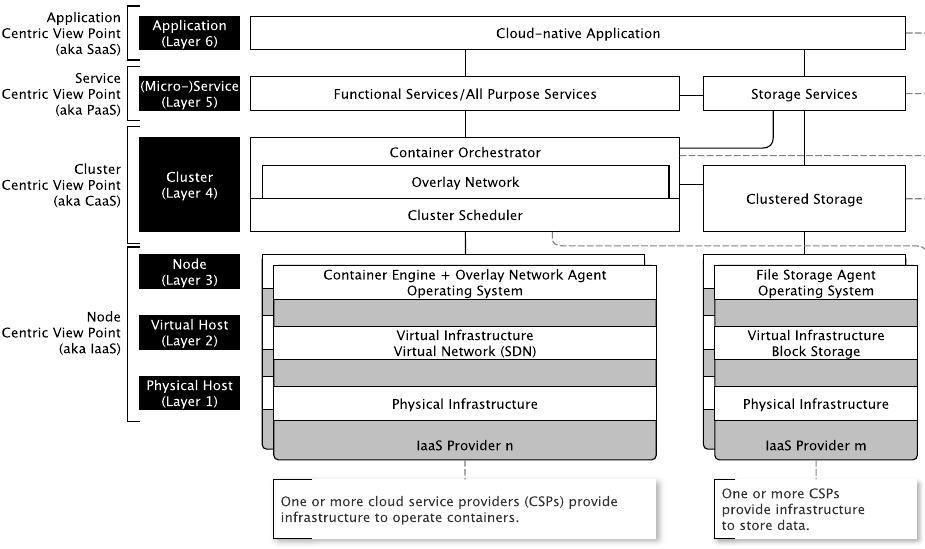
\includegraphics[width=\textwidth]{img/ClouNS_Stack.png}
    \caption[Der ClouNS Stack]{Der ClouNS Stack\cite{kratzke_clouns_2016}}
    \label{fig:clouNS}
\end{figure}

\subsection{Infrastructure as a Service (IaaS)}
Infrastructure as a Service bietet die Grundlage des Cloud Native Stacks. Einem Kunden werden hierbei grundlegende zumeist virtualisierte Hardware-Ressourcen wie Prozessorleistung, Speicher oder Netzwerkmöglichkeiten angeboten. Auf diesen kann er seine Software beliebig ausführen. Er hat dabei keinen Einfluss auf die zugrundeliegende Cloud Infrastruktur (also die Server-Pools an sich), aber kann Betriebssysteme, Anwendungen und verwendeten Speicher kontrollieren\cite{mell_nist_2011}. \\

\subsection{Cluster as a Service (CaaS)}
Bei Cluster as a Service handelt es sich um eine Schicht über IaaS, die ein Clustering von Containern bietet. Hier agieren Orchestrierungs Tools wie zum Beispiel Kubernetes, die Container auf das Cluster verteilen, skalieren und managen\cite{kratzke_clouns_2016}. \\

\subsection{Platform as a Service (PaaS)}
Eine höhere Abstraktionsebene über IaaS oder CaaS. Einem Kunden wird auch hier die Kontrolle über die in der Cloud Infrastruktur auszuführende Anwendung gegeben. Allerdings kann er nicht über verwendete Betriebssysteme, Speichernutzung, Netzwerkkonfiguration usw. entscheiden. Dafür werden ihm vom Anbieter Programmier- oder Laufzeitumgebungen, Tools und Bibliotheken angeboten, die die Entwicklung und Ausführung der Anwendung auf der Infrastruktur ermöglichen\cite{mell_nist_2011}.\\

\subsection{Software as a Service (SaaS)}
Eine höhere Abstraktionsebene über PaaS. Einem Kunden werden hier vom Anbieter explizite auf Cloud Infrastruktur auszuführende Anwendungen bereitgestellt, die dieser verwenden kann. Der Kunde hat weder Einfluss auf die zugrundeliegende Cloud Infrastruktur, noch auf verwendete Betriebssysteme oder Software. Die Ausnahme bilden limitierte Einstellungsmöglichkeiten der vom Anbieter bereitgestellten Anwendung\cite{mell_nist_2011}.

\section{Cloud Native Computing}
Cloud Native Technologien oder Cloud Native Computing ist laut der Cloud Native Computing Foundation (CNCF) eine Ansammlung von Technologien, die es Unternehmen ermöglichen "`skalierbare Anwendungen in modernen, dynamischen Umgebungen zu implementieren und zu betreiben"' \cite{noauthor_cncftoc_nodate}. Bei diesen dynamischen Umgebungen handelt es sich dabei ausschließlich um Cloud Umgebungen (also private, öffentliche und hybride Clouds). Diese Systeme sollen lose gekoppelt, "`belastbar, handhabbar und beobachtbar"' sein und durch Automatisierung schnelle Änderungen ermöglichen\cite{noauthor_cncftoc_nodate}.

\section{Containerisierung}
Containerisierung ist eine Technik, den Code einer Anwendung mitsamt aller Abhängigkeiten, die diese zur Ausführung benötigt, zu verpacken. Ein solches Paket wird als Container Image bezeichnet. Da alle Abhängigkeiten enthalten sind, werden dadurch die Laufzeitunterschiede auf unterschiedlichen Plattformen minimiert\cite{noauthor_what_nodate}. Zur Laufzeit wird ein Container Image als Container bezeichnet. Um ein Container Image auszuführen, wird eine Container Runtime benötigt. Die erste Container Runtime Engine wurde von Docker entwickelt, wird aber mittlerweile als Open-Source Projekt mit dem Namen containerd von der Open Container Initiative (OCI) betrieben\cite{noauthor_what_nodate}. 

Containerisierte Anwendungen unterscheiden sich von Virtuellen Maschinen vor allem darin, dass kein Hypervisor zur Ausführung der Images benötigt wird. Stattdessen teilen sich alle Container das Host-Betriebssystem und werden in einem eigenen User-Space isoliert. Dadurch können Container-Images deutlich leichtgewichtiger und schneller als Virtuelle Maschinen ausgeführt werden. Abbildung \ref{fig:containerVsVMs} verdeutlicht nochmals den Unterschied beider Technologien.

\begin{figure}[H]
    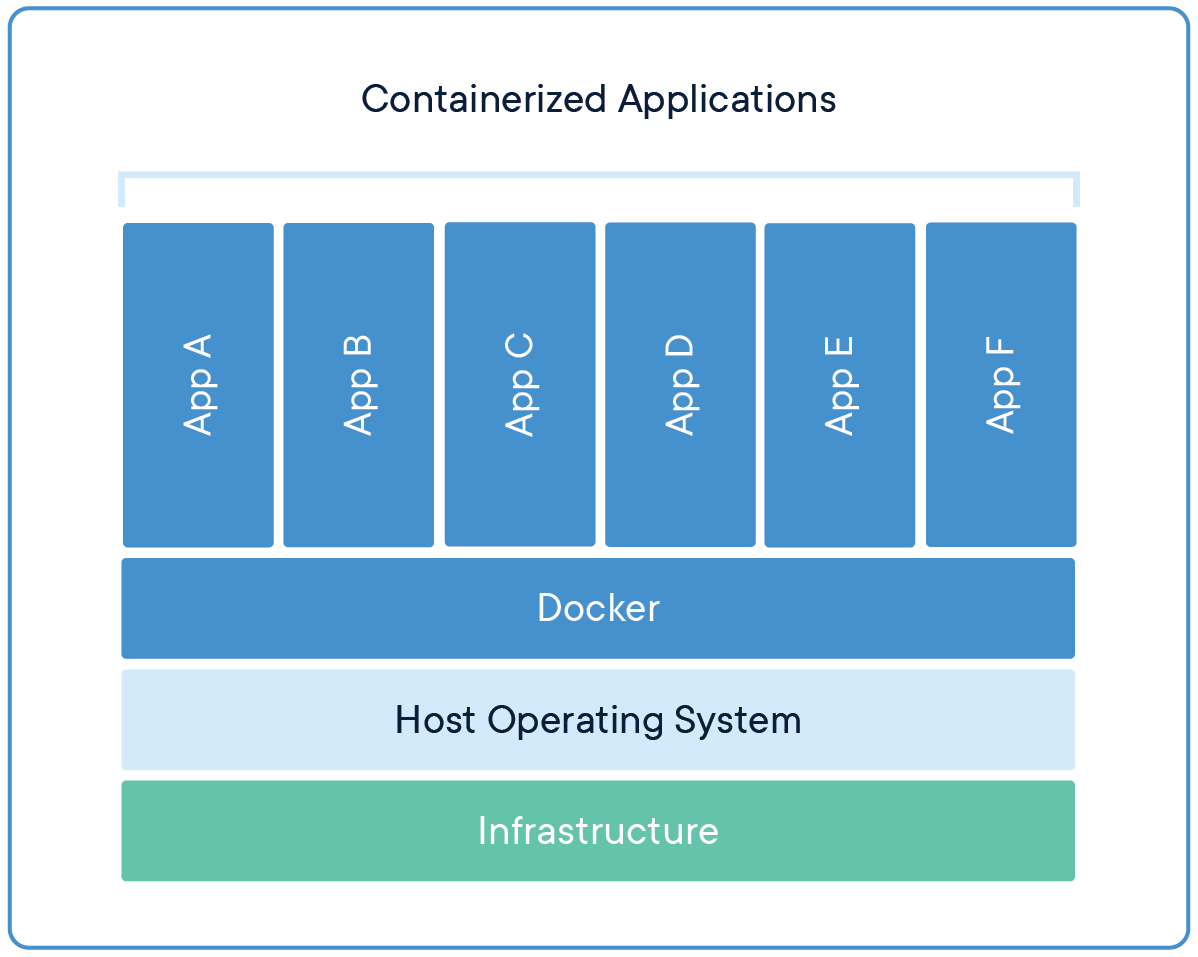
\includegraphics[width=200pt]{img/container-architecture.png}
    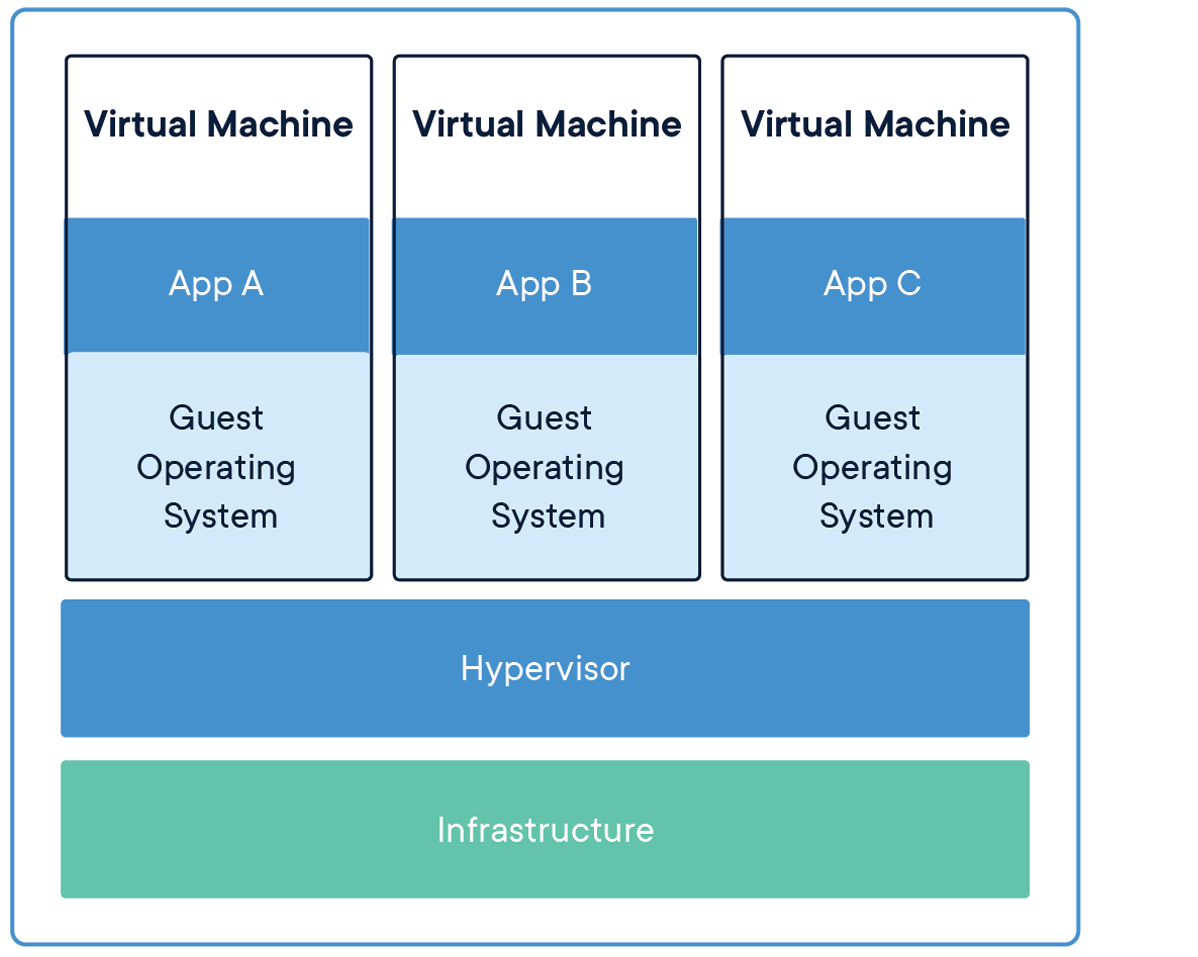
\includegraphics[width=200pt]{img/vm-architecture.png}
    
    \caption[Vergleich zwischen Containern und Virtuellen Maschinen]{Vergleich zwischen Containern und Virtuellen Maschinen\cite{noauthor_what_nodate}}
    \label{fig:containerVsVMs}
\end{figure}

\section{Container-Orchestrierung}
Container-Orchestrierung beschreibt die Automatisierung der "`Bereitstellung, Verwaltung, Skalierung und Vernetzung von Containern"'\cite{noauthor_was_nodate-1}. Mit Orchestrierungs-Tools wie Kubernetes, lassen sich Container einfach auf Computer-Clustern provisionieren, skalieren und überwachen. Wie im ClouNS Modell (Abb. \ref{fig:clouNS}) zu sehen ist, agieren Container Orchestrierungs Tools auf der CaaS Ebene. Dadurch erlauben sie das Betreiben von infrastrukturunabhängigen und flexiblen Anwendungen auf Basis von Containern\cite{noauthor_was_nodate}.

\section{Serverless}
Serverless ist ein Software-Ausführungsmodell, bei dem ein Cloud Anbieter (z.B AWS, Azure, GCP) sich vollständig um die Ausführung einer Anwendung inklusive Konfiguration der zugrundeliegenden Server kümmert. Der Programmierer kann sich daher ausschließlich auf das Schreiben des Codes konzentrieren und muss keine Zeit in das Einstellen und Aufsetzen von Servern investieren. \\
Dabei wird die Software in einem Stateless-Container, d.h einem Container ohne persistentem Speicher, ausgeführt. Der Cloud-Anbieter stellt dabei die Ressourcen dynamisch bzw. on-demand bereit, d.h die Anwendung wird nur dann ausgeführt, wenn eine diesbezügliche Anfrage eintrifft. Serverless verspricht dadurch eine effizientere Entwicklung und Kosteneinsparungen, da bei den Anbietern nur der tatsächlich laufenden Code abgerechnet wird. In der Regel muss vom Entwickler einer Serverless-Anwendung nur eine einzige Funktion geschrieben werden, weshalb Serverless auch als Function-as-a-Service (FaaS) bezeichnet wird\cite{noauthor_was_2016}. \\
Da eine Serverless-Funktion nicht dauerhaft ausgeführt wird, muss bei einem eingetretenen Event erst einmal der Anwendungscontainer aufgesetzt werden. Dies wird als "`Cold Start"' bezeichnet und kann sich als Latenz bei der Ausführung der Funktion bemerkbar machen. Ist der Container einmal gestartet kann er von den Cloud-Anbietern vorgehalten werden und bei der nächsten Anfrage schneller reagieren. Dies wird auch als "`Warm Start"' bezeichnet\cite{noauthor_was_2016}. Es gibt einige Techniken, um seine Funktionen möglichst warm zu halten, die auch in dieser Arbeit untersucht werden.
\chapter{Related Work}
In diesem Kapitel werde ich verwandte Arbeiten vorstellen.

\section{Literatur}
Serverless ist allgemein ein noch junges Thema, das erst mit der Einführung von AWS Lambda im Jahre 2014 viel Aufmerksamkeit erfuhr. Es gibt bereits einige Studien zu der Performance von Serverless-Anwendungen, jedoch wurde in den meisten Studien nur Micro-Benchmarks betrachtet, d.h Tests, die nur einen Aspekt untersuchen, bspw. die CPU-Floating-Point Performance und keine realistischen Applikationen untersuchen\cite{scheuner_function-as--service_2020}. Vergleiche mit der Performance von Container-Anwendungen sind nur sehr wenige zu finden. 
In "`Serverless computing: Design, implementation, and performance"'\cite{mcgrath_serverless_2017} wurden mehrere Tests zur Performanz von Serverless-Funktionen durchgeführt. Unter anderem wurde ein Nebenläufigkeits-Test (concurrency test) vorgestellt, bei dem eine Funktion, die sofort terminiert, von einer linear ansteigenden Anzahl an Clients so oft wie möglich hintereinander aufgerufen. Gemessen wurde dabei die Anzahl der Antworten pro Sekunde (responses per second). Ziel dieses Tests war, die performante Ausführung einer skalierten Funktion zu messen. Das Ergebnis zeigte unterschiedliches Skalierverhalten für diverse Cloud-Anbieter; bei AWS Lambda wurde jedoch ein weitestgehend linearer Anstieg festgestellt. 
Des Weiteren werden für zukünftige Forschung noch andere die Performanz von Serverless-Funktionen beeinflussende Aspekte genannt, wie die Ausführung mehrerer Funktionen anstatt nur einer einzigen (single function execution), die Code-Größe einer Serverless-Funktion und unterschiedliche CPU-Allokation (in der Studie wurde lediglich 512MB RAM verwendet).

Das Paper "`Serverless computing: Design, implementation, and performance"'\cite{hendrickson_serverless_2017} vergleicht die Performance von AWS Lambda mit der eines in AWS Beanstalk laufendem Docker-Containers. Dazu sendeten die Forscher jeweils 100 RPC-Requests an beide Services, wobei jeder Service eine Laufzeit von 200ms beanspruchte. Die Durchführung des Tests ergab, dass die Antwortzeit bei Lambda mit einem Medianwert von 1,6 Sekunden deutlich vor der von Beanstalk mit bis zu 20 Sekunden liegt. Als Grund dafür wird angeführt, dass Lambda innerhalb von einigen Millisekunden 100 Instanzen auf die der Last verteilt wurde, während bei Beanstalk alle Anfragen von einer einzigen Instanz bearbeitet wurde, obwohl alle Einstellungen getroffen wurden, damit Beanstalk so schnell wie möglich hochskalieren kann. Hier zeigen sich deutlich die automatischen Skalierungsvorteile einer FaaS Applikation. Während es bei Beanstalk 20 verschiedene Einstellungsmöglichkeiten gäbe, übernimmt Lambda dies vollkommen automatisch.
Allerdings wird auch deutlich, dass die Latenz von Lambda Funktionen bei einer normalen Last deutlich über der eines Containers liegt. Mit der gleichen Testumgebung und unter leichter Last, performe Lambda 10 mal schlechter als Beanstalk. Da dieser Test im Jahre 2017 durchgeführt wurde, stimmen diese Ergebnisse aber vermutlich nicht mit den in der Zwischenzeit an Lambda vorgenommenen Performance-Verbesserungen überein.

Das Paper "`Infrastructure cost comparison of running web applications in the cloud using aws lambda and monolithic and microservice architectures"'\cite{villamizar_infrastructure_2016} vergleicht die Performance und infrastrukturellen Kosten einer auf verschiedene Arten deployten Applikation. Die Anwendung wurde als Monolith und als Microservices mit und ohne AWS Lambda betrieben. Dabei zeigte sich,  dass die Kosten für den Betrieb bei einer auf Lambda basierten Microservices Architektur deutlich (mehr als 70 Prozent) geringer ausfallen können, als bei einem Monolith oder wenn die Microservices von den Entwicklern selbst gemanaged werden. Ebenfalls wurde die Performance der verschiedenen Ansätze mittels der Metrik der durchschnittlichen Antwortzeit (average response time - ART) verglichen. Es wurde deutlich, dass Lambda in unterschiedlichen Test-Szenarien nahezu die gleich ART beibehält, was auf dessen Skalierungsmöglichkeiten zurückgeführt wurde. Des Weiteren performte Lambda teilweise besser als die monolithische Architektur und deutlich besser als die selbst-gemanagten Microservices.

\chapter{Konzeption}
In diesem Kapitel werde ich die grundlegende Konzeption der Arbeit vorstellen.

\section{Methodisches Vorgehen}
Es soll eine Beispielanwendung sowohl Containerisiert als auch Serverless entwickelt werden. Die Konzeption dieser beiden Anwendungen wird in den folgenden Abschnitten genauer beschrieben. 
Im Anschluss werden Performance Tests gegen beide Anwendungen durchgeführt und die Ergebnisse miteinander verglichen. Das methodische Vorgehen basiert dabei grundlegend auf den von Papadopoulus et. al. vorgestellten methodologischen Prinzipien für reproduzierbare Performanz-Evaluation im Cloud Computing Umfeld, die im folgenden beschrieben werden\cite{papadopoulos_methodological_2019}:

\begin{enumerate}
    \item[P1] Wiederholte Durchführung (Repeated experiments): Festlegen, wie viele Experimente mit der selben Konfiguration gemacht werden sollten. 
    \item[P2] Konfigurations-Abdeckung (Workload and configuration coverage): Experimente in verschiedenen Konfigurationen der relevanten Parameter durchführen. Beispielsweise verschiedene Hardware-Konfigurationen aber auch verschiedene Load-Testing-Typen (z.B. Spike Test)
    \item[P3] Experimenteller Aufbau (Experimental setup description): Beschreibung der Hardware- und Software (inklusive Version), und anderer Parameter die für das Experiment genutzt wurden und einen Einfluss auf dessen Ausgang haben können. Zusätzlich sollte die Beschreibung das genaue Ziel des Experiments beinhalten.
    \item[P4] Offener Zugang zu Artefakten (Open access artifact): Möglichst viele für die Experimente genutzten Konfigurationsdateien, Protokolle, etc. sollten versioniert und offen zugänglich sein.
    \item[P5] Probabilistische Ergebnisbeschreibung der gemessenen Performanz (Probabilistic result description of measured performance): Angemessenes Beschreiben und Visualisieren der Ergebnisse. Verwendung von Quantilen (z.B. Median oder 95. Quantil) und der Standardabweichung.
    \item[P6] Statistische Auswertung: Statistische Tests anwenden, um die Validität der Studie zu untermauern. Dieses Prinzip wird aus mangelnder Expertise und Zeit nicht genauer betrachtet, daher hier der Hinweis, dass die Ergebnisse dieser Arbeit eventuell nicht signifikant sind.
    \item[P7] Einheiten (Measurement units): Für alle Messungen die zugehörige Einheit angeben
    \item[P8] Kosten (Cost): Kostenmodell, Ressourcennutzung und abgerechnete Kosten angeben.
\end{enumerate}

\section{Konzeption der Testanwendung}
Als Testanwendung wird ein einfaches REST-Backend am Beispiel eines Notiz-Applikation entwickelt, wie es in der Praxis häufig verwendet wird. Der Service stellt folgende Routen bereit:  

\begin{enumerate}
    \item GET /notes: Das Auflisten aller verfügbarer Notizen
    \item GET /notes/\{id\}: Das Auflisten eines spezifischen Notiz mit der angegebenen id
    \item PUT /notes/\{id\}: Das Ändern einer spezifischen Notiz mit der angegebenen id
    \item POST /: Das Erstellen einer Notiz
\end{enumerate}

Um die Anwendung möglichst einfach zu gestalten und Unterschiede zwischen den beiden Technologien zu minimieren, wird zunächst auf die Verwendung einer Datenbank verzichtet. Stattdessen wird ein Delay von 50 Millisekunden für jeden Request eingebaut. 
Auch auf Authorisierungs-Mechanismen wird der Einfachheit halber verzichtet. Dies erlaubt es außerdem, von einer konstanten Benutzer-Rate auszugehen\cite{molyneaux_art_2014}. 
Als Runtime wird sowohl bei der Serverless- als auch bei der containerisierten Anwendung Node.js 12 verwendet.

\subsection{Serverless}
Für die Entwicklung der Serverless-Anwendung wird das, mit mehr als 38.000 Github-Stars populäre, Serverless-Framework\cite{noauthor_serverless_nodate} verwendet. Dabei handelt es sich um ein Open-Source Framework zur Entwicklung von Serverless Anwendungen. Es übernimmt die Erstellung von Anwendungs-Stacks, Rechteverteilung und Konfiguration bei allen gängigen Public-Cloud Anbietern wie AWS, Azure oder GCP. Da in dieser Arbeit AWS verwendet wird, erstellt Serverless automatisch einen Anwendungs-Stack mit AWS CloudFormation. Dabei wird ein AWS API-Gateway erstellt, das über die Routen der REST-Schnittstelle verfügt. Trifft eine Anfrage an eine der Routen ein, übernimmt das API-Gateway die Auslösung des passenden Events, wodurch die korrekte Lambda-Funktion mit den vom Benutzer im HTTP-Request übergebenen Parametern aufgerufen wird. 

Durch die Nutzung des Frameworks wird die Erstellung der Anwendung vereinfacht. Denn auch wenn man sich nicht mehr um Server kümmern muss, ist dennoch die Konfiguration des API-Gateways notwendig.

Abbildung \ref{fig:notes-serverless} zeigt das Setup der mit der Serverless-Architektur konzipierten Webanwendung.

\begin{figure}[H]
    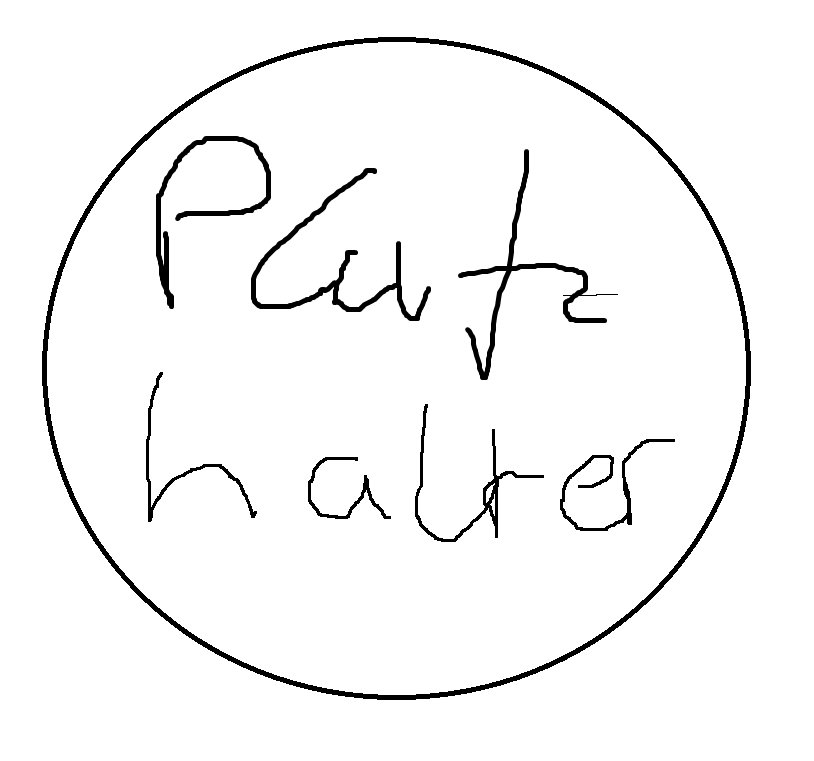
\includegraphics[width=\textwidth]{img/platzhalter.png}
    \caption[Serverless Notiz-Anwendung]{Serverless Notiz-Anwendung}
    \label{fig:notes-serverless}
\end{figure}

\subsection{Container}
Für die Entwicklung der containerisierten Anwendung wird das Express Framework verwendet, das mit über 51.000 Github-Stars eines der meist verwendeten Web-Frameworks für Node.js ist. Die Anwendung wird unter Nutzung der Docker-Engine mittels einer Dockerfile in ein Container-Image gebaut. Dieses Image wird in der AWS Elastic Container Registry (ECR) gespeichert, um es von dort aus weiter zu verwenden. 
Die Ausführung der Anwendung erfolgt auf der AWS Elastic Container Service (ECS) Plattform, einem von AWS bereitgestelltem Orchestrations-Tool. Es wird AWS Fargate benutzt, um die Erstellung eines Server-Clusters weg zu abstrahieren. Des Weiteren wird ein Elastic Load Balancer (ELB) vom Typ Application verwendet, um die eingehenden Requests auf die verschiedenen Container zu verteilen. 

Abbildung \ref{fig:notes-container} zeigt das Setup der mit der Container-Architektur konzipierten Notiz-Anwendung.

\begin{figure}[H]
    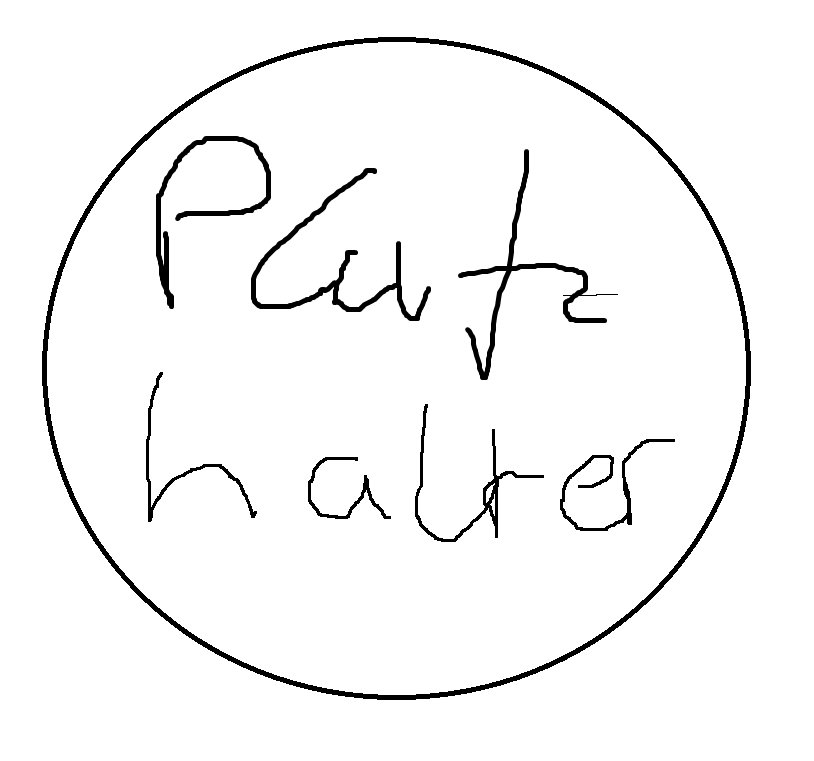
\includegraphics[width=\textwidth]{img/platzhalter.png}
    \caption[Containerisierte Notiz-Anwendung]{Containerisierte Notiz-Anwendung}
    \label{fig:notes-container}
\end{figure}

\section{Konzeption der Tests}

\subsection{Testing-Tool}
Um die Performance der eben vorgestellten Anwendungen zu testen, wird das Performance-Testing Tool k6 \cite{noauthor_load_nodate} verwendet. Durch eine optimierte CPU Auslastung ermöglicht es, etliche virtuelle Benutzer zum Testen einer Anwendung erstellen lassen ohne die Notwendigkeit einer verteilen Ausführung\cite{noauthor_running_nodate}. Die Benutzer arbeiten parallel die in Sektion \ref{sec:use-cases} vorgestellten Use-Cases ab, bei denen verschiedene Requests an die REST-APIs der Services geschickt werden. 

Als Load-Generator wird eine in der AWS Region Paris (eu-west-3) stationierte EC2 Instanz des Typs t3.large verwendet.
Nach eigenen Angaben benötigt k6 für jeden virtuellen Benutzer und für einen kleinen Test eine Speicherauslastung zwischen 1 und 5 Megabyte\cite{noauthor_running_nodate}. Da die verwendete t3.large Instanz 8 Gigabyte RAM beinhaltet, sollten theoretisch mehr als 1600 und maximal 8000 gleichzeitige virtuelle Benutzer von der Testumgebung unterstützt werden. Die Instanz weist eine Netzwerkleistung von bis zu 5 Gbit/s auf, welche bei jeder Testausführung mittels des Tools iftop überwacht wird, um sicherzugehen, dass das Netzwerk nicht zum Flaschenhals wird. Auch die CPU Auslastung wird mittels htop überprüft.

\subsection{Metriken}
Das Testing-Tool k6 speichert für jeden Request an einen bestimmten API-Endpunkt unter anderem Werte folgender Metriken:
\begin{enumerate}
    \item VUS (virtual users): Die Anzahl der virtuellen Benutzer zum aktuellen Zeitpunkt 
    
    \item Response Time: Die Zeit vom Abschicken eines Requests bis zum Erhalt der Antwort in Millisekunden (ms). Dabei wird Aufwand für eventuelle DNS Lookups nicht mit einberechnet. 
    
    \item HTTP-Statuscodes: Geben den Status eines HTTP-Requests an. Wichtig für die Betrachtung sind vor allem die Codes:
        \begin{enumerate}
            \item 200 (OK): Der Request war erfolgreich.
            \item 503 (Service Unavailable): Der Server kann den Request nicht bearbeiten. Kann auftreten, wenn zu viele Requests bei einem Service eintreffen und dieser aufgrund mangelnder verfügbarer Ressourcen (CPU / Speicher) nicht in der Lage ist, die Anfrage zu bearbeiten.
        \end{enumerate}
        
    \item Request Rate: Die aggregierte Anzahl aller bereits abgeschlossenen Requests pro Sekunde (req / s)
\end{enumerate}

Da k6 keine eingebaute Visualisierungslösung bietet, werden diese Werte mittels der k6 Integration an den Cloud-Monitoring Service Datadog gesendet. Dort treffen sie mit von AWS Cloudwatch gesammelten Metriken zusammen, wodurch sie gemeinsam ausgewertet werden können.

Abbildung \ref{fig:test-architecture} zeigt das vollständige Setup der mit der Testing-Architektur.

Für zusätzliche Analysen und Vergleiche mehrerer Test-Ausführungen untereinander, werden die Ergebnisse jedes k6-Tests auch als CSV-Text-Datei exportiert. Im Anschluss können diese Dateien mit dem Data-Science Framework Pandas\cite{noauthor_pandas_nodate} für die Programmiersprache Python analysiert und verglichen werden. Der Source-Code der Analysen und die Ergebnis-Artefakte der Tests sind im Code-Repository dieser Arbeit zu finden.
\begin{figure}[H]
    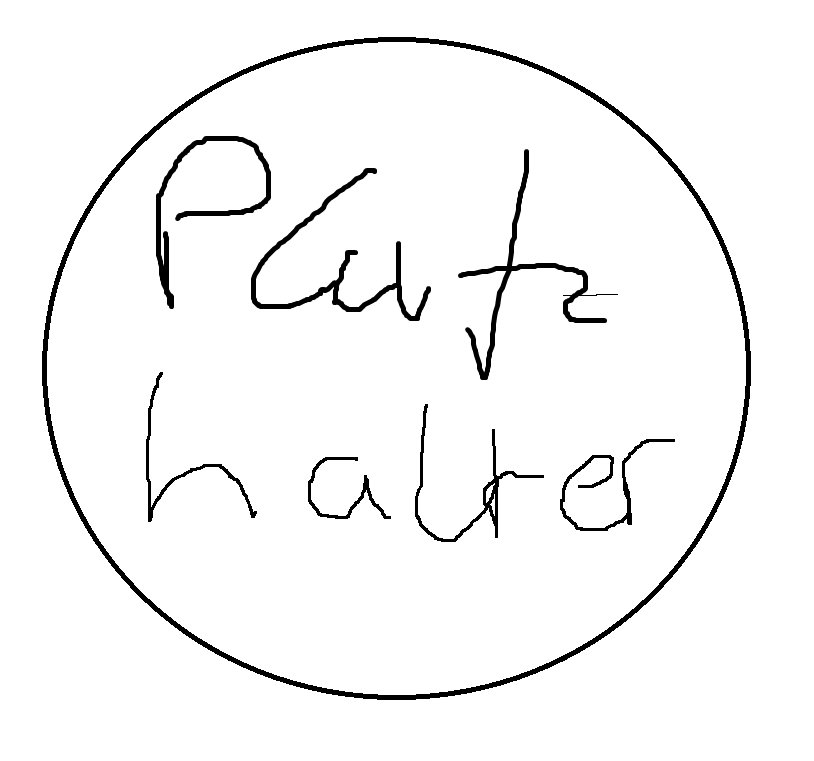
\includegraphics[width=\textwidth]{img/platzhalter.png}
    \caption[Test Architektur der Notiz-Anwendung]{Test Architektur der Notiz-Anwendung}
    \label{fig:test-architecture}
\end{figure}

\subsection{Test-Typen}
Bei Performance Tests können verschiedene Testing-Strategien eingesetzt werden.
\begin{enumerate}
    \item Load Testing: Dient der Evaluierung der System-Performance in Bezug auf die Anzahl der gleichzeitigen Benutzer oder der Requests-Rate. Es wird der Normalbetrieb des Systems simuliert.
    
    \item Stress Testing: Dient dazu, die Grenzen des Systems in den Punkten Verfügbarkeit und  Stabilität auszutesten. Man geht über den normalen Betrieb hinaus und eventuell so hoch dass das System der Last nicht mehr standhalten kann. Bei einem Stress-Test wird schrittweise die Last auf das System erhöht. So kann man zum Beispiel herausfinden, ob das System großen Anstürmen, wie z.B einem Sale-Event bei einem Online-Shop, Stand halten kann.
    
    \item Spike Testing: Eine Variante des Stress-Tests bei dem in einem kurzen Zeitraum extreme Last für das System-under-Test generiert wird. Im Gegensatz zu einem normalen Stress-Test, wird die Last hierbei nicht stufenweise, sondern plötzlich erhöht. Dadurch wird getestet, wie das System reagiert, wenn nicht ausreichend Zeit zur Skalierung der Infrastruktur bekommt.
\end{enumerate}

Es gibt noch weitere Test-Typen wie Smoke- oder Soak-Tests, die allerdings keine Relevanz für die Zielfrage dieser Arbeit haben und daher nicht betrachtet werden.

\subsection{Getestete Use-Cases}\label{sec:use-cases}
Die folgenden Use-Cases werden bei der Analyse der Systems-under-test evaluiert. Die nach einem Request angegebenen Zeitintervalle entsprechen der sogenannten "`Think Time"', also der Zeit die ein Benutzer normalerweise benötigt um sich für seine nächste Handlung zu entscheiden. Es wird, wie von Molyneaux empfohlen, mit einer ±10 prozentigen Abweichung versucht, eine realistischere Szenariodurchführung zu erreichen\cite{molyneaux_art_2014}.
\begin{itemize}
    \item Use-Case A: Alle Notizen abrufen \\
        Alle Notizen einmal abrufen. \\
        1. GET /notes -> 2s     \\

    \item Use-Case B: Notiz bearbeiten \\
        Erst alle Notizen, dann eine einzelne Notiz abrufen und bearbeiten. \\
        1. GET /notes -> 2s     \\
        2. GET /notes/1 -> 5s   \\
        3. PUT /notes/1         \\
        
    \item Use-Case C: Notiz falsch erstellt \\
    Der Benutzer ruft alle Notizen ab. Er entscheidet sich eine Notiz erstellen. Er ruft die erstellte Notiz ab und bemerkt dass er einen Fehler gemacht hat. Er bearbeitet die Notiz und speichert die Notiz erneut ab. \\
        1. GET /notes   -> 10s  \\
        2. POST /notes  -> 3s   \\
        3. GET /notes/1 -> 5s   \\
        4. PUT /notes/1
\end{itemize}


\subsection{Test-Variablen}
\begin{itemize}
    \item Use-Case: A / B / C
    \item Test Typ: Pipe-clean, Load, Stress, Spike-Test
    \item CPU und Memory des Systems: 128-...
    \item Skalierungs-Größe: 2 / 3 / 5 / 10 Task-Instanzen
    \item Anzahl an parallelen Benutzern: 25 / 50 / 75 / 100 ... 200
    \item Größe der Lambda Funktion
    \item Unterschiedliche Szenarien: Bei Lambda großer Unterschied 

    \item (Datenbank -> vielleicht Einfluss auf Memory?)
    \item (Skalierungs-Schwellen: Ab 60 / 70 / 75 Prozent CPU Auslastung)
    \item (Minimiertes JavaScript)
\end{itemize}


Es ergeben sich dadurch folgende Test-Szenarien:

CPU 128 / 256 / 512 für Use-Case A / B / C mit Instanzen 1 / 2 / 3 

\subsection{Test-Ablauf}
Nach Molyneaux \cite{molyneaux_art_2014} sollte zunächst ein Pipe-clean Test durchgeführt werden. Dabei wird jedes System von nur einem einzigen Benutzer für ein bestimmtes Szenario angefragt. Dadurch lassen sich Basiswerte für die betrachteten Metriken ableiten, welche in späteren Tests zu Vergleichen hinzugezogen werden können.

Anschließend wird ein Stress-Test für die Konfiguration der Container-Anwendung durchgeführt. Dies ist notwendig, da AWS Lambda ein von Natur automatisch skalierendes System ist, während ein Container alleine nicht skalieren kann. Um eine zu hohe Auslastung des Containers während des Tests zu vermeiden, wird der Stress-Test durchgeführt, um das VU-Limit für die aktuelle Container-Konfiguration zu erkennen. 
Im Anschluss wird mit diesem ermittelten VU-Limit ein Last-Test gegen beide System durchgeführt und die Ergebnisse beider SUTs miteinander verglichen.

\chapter{Analyse}
In diesem Kapitel werden die in Kapitel 3 vorgestellten Analysen durchgeführt. Die Forschungsfrage wurde in kleinere Teilfragen aufgeteilt, die im folgenden untersucht werden sollen:

\begin{enumerate}
    \item[RQ1] Wie vielen nebenläufige Lambda-Funktionen werden benötigt, um den maximalen Load einer einzigen Container-Instanz zu tragen?
    
    \item[RQ2] Wie ist die Performance bei normalem Load oder bei Spike Load? \\
    H1: Die Performance einer Lambda Funktion stagniert unter Spike Load stark, während sie bei einem Container gleich bleibt.

    \item[RQ3] Welchen Einfluss hat die Nutzung größerer CPU / RAM Werte? \\
    H3: Ein Container kann bei einer Verdopplung doppelt so viele Anfragen verarbeiten. Eine Lambda Funktion kann ihre Anfragen schneller verarbeiten.
    
    \item[RQ4] Welchen Einfluss hat die Nutzung mehrerer Container Instanzen auf die Performance? \\
    H4: Die Performance steigt linear mit jedem neuen Container an
    
    \item[RQ5] Welchen Einfluss hat die ein Use-Case, der mehreren Endpunkten anfragt\\
    H5: Bei Lambda großer Einfluss, da jede Funktion einzeln einen Coldstart machen muss
\end{enumerate}

\section{Pipe-Clean Tests}
Zunächst wird die Performance der SUTs in der bestmöglichen Situation mit einem einzigen Nutzer ermittelt. Ziel dessen ist es, eine Vergleichsgrundlage für die darauf folgenden Tests zu schaffen. Der Test wurde mit einer Dauer von zehn Minuten mit einem aktiven Benutzer für jeden Use-Case durchgeführt. Jeder Test wurde drei mal ausgeführt und die Metriken über die Gesamtmenge der Daten aggregiert. Bei den Requests wurde die Summe gebildet, bei den durchschnittlichen Requests pro Sekunde das arithmetische Mittel.

\begin{figure}[H]
    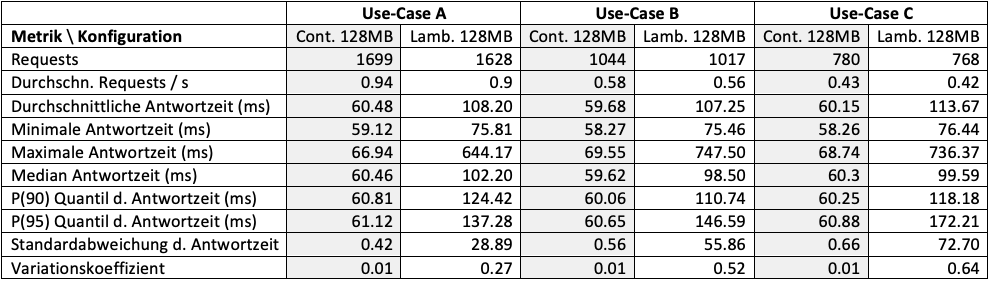
\includegraphics[width=\textwidth]{img/pipe128-comparison.png}
    \caption[Vergleich der Pipe-Clean Tests für 128MB]{Vergleich der Pipe-Clean Tests für 128MB}
    \label{fig:pipe128-comparison}
\end{figure}

Abbildung \ref{fig:pipe128-comparison} zeigt die Ergebnisse des Tests für die Funktionen mit 128MB CPU bzw. RAM. Es ist zu erkennen, dass die Container Anwendung in allen Fällen eine deutlich geringere Antwortzeit als die Lambda Anwendung aufweist. Im Median ist der Container bei Use-Case A etwa 41,74ms schneller als die Lambda-Funktion. Während die maximale Antwortzeit bei ersterer nur etwa 10,7\% über dem Median liegt, ist sie bei der Lambda-Funktion etwa 630\% über ihrem Median. Dass die Lambda-Anwendung eine überaus große Varianz in ihren Antwortzeiten aufweist, wird auch in ihrer Standardabweichung von bis zu 72ms deutlich, währende sie bei der Container Anwendung in allen drei Use-Cases unter 1ms liegt. Interessanterweise liegt die Antwortzeit der Lambda-Anwendung im Median in allen drei Use-Cases bei ähnlichen Werten um ca. 100ms. Andererseits nimmt die Standardabweichung und das P(95) Quantil der Antwortzeit bei Use-Case B im Vergleich zu Use-Case A deutlich zu. Und auch bei Use-Case C ist ein deutlicher Anstieg der Werte zu beobachten. Vermutlich ist dies auf die größere Anzahl an angefragten Endpunkten zurückzuführen, da dadurch mehr Coldstarts durchgeführt werden müssen. Auch bei der Container-Anwendung ist keine Veränderung der Median-Antwortzeit um ca. 60ms festzustellen. Die Standardabweichung der Antwortzeit erhöhte sich nur leicht von 0,42 auf 0,66.

\section{128MB Konfigurationen}
Zunächst werden alle Tests gegen die 128MB Konfigurationen ausgeführt. In den folgenden Sektionen wird dann die Speicher- und Prozessorgröße erhöht. 

\subsection{Stress-Tests}
Um RQ1 zu beantworten, muss zunächst die maximale Auslastung eines einzelnen Containers ermittelt werden. Dazu wurden mehrere Stress-Tests durchgeführt. Ein Stress-Test dient dazu, die Grenzen des SUTs herauszufinden. Da Lambda ein von Natur aus automatisch horizontal skalierendes System ist, werden die Test zunächst für die Container-Anwendung durchgeführt und im Anschluss die Lambda-Anwendung mit der gleichen Test-Konfiguration getestet. Dadurch kann das Verhalten der Funktionen bei langsamem Anstieg der Benutzer evaluiert werden. Die Anzahl der VUs wird bei den Stress-Tests wie von Molyneaux\cite{molyneaux_art_2014} empfohlen immer stufenweise erhöht. Das bedeutet, dass nach jedem Ramp-Up (ein linearer Anstieg) eine gleichlange Periode mit einer konstanten Anzahl an Benutzern folgt. Abbildung \ref{fig:stress-vus-example} verdeutlicht dies anhand eines Stress-Tests, bei dem bis zu 600 gleichzeitige Virtuelle Benutzer erstellt werden. In 60 Sekunden Zeitabschnitten werden nach und nach immer 60 Benutzer hinzugefügt. Daraufhin folgt eine weitere 60 Sekunden lange Periode, in der die Anzahl der VUs nicht weiter erhöht wird. Der gesamte Test hat demnach eine Dauer von 40 Minuten. Eine Cooldown-Phase nach den vollen 600 Benutzern wird hier nicht eingelegt, da das Skalierungsverhalten nicht untersucht wird.

\begin{figure}[H]
    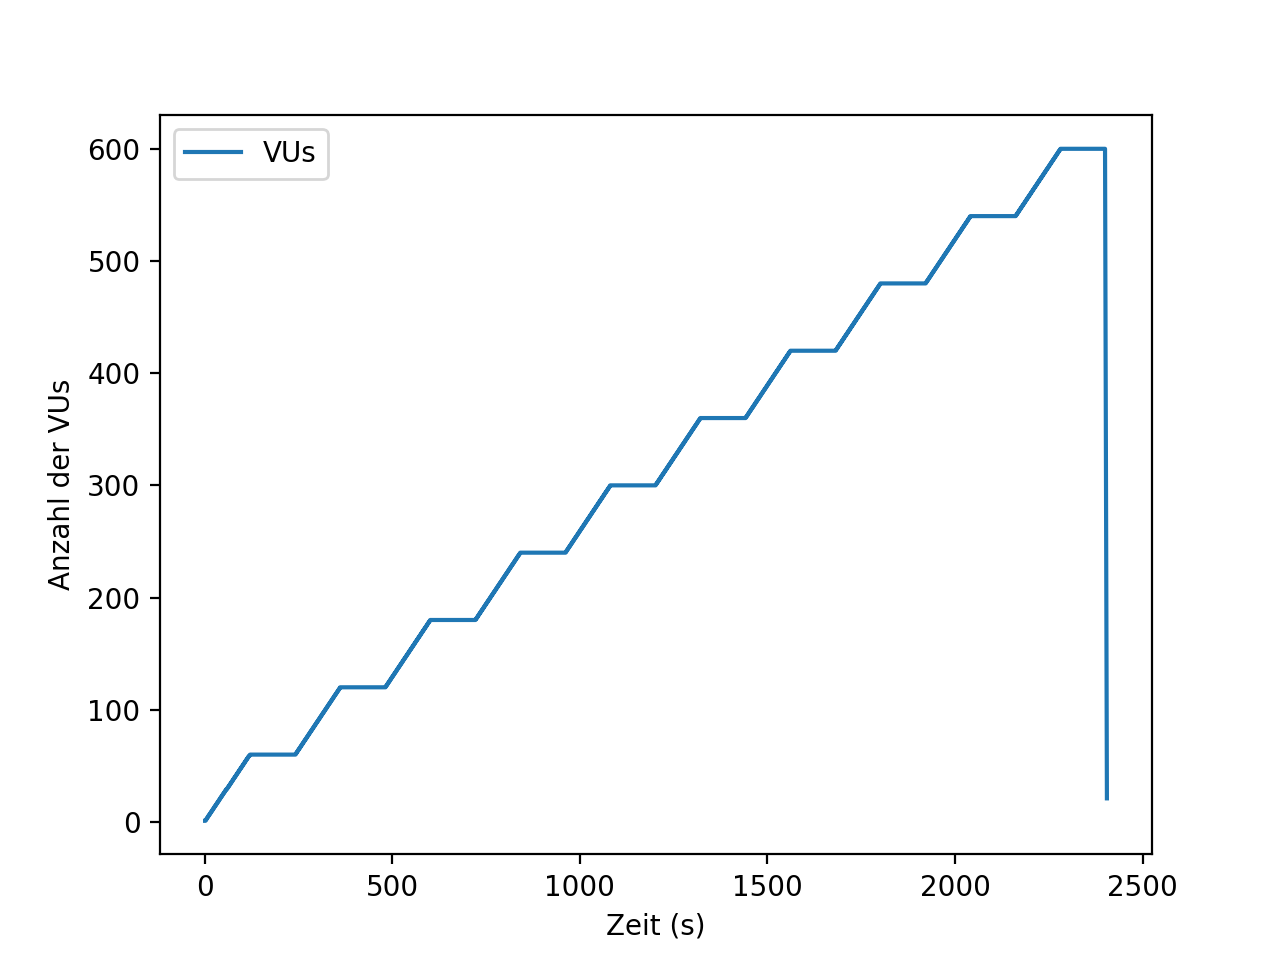
\includegraphics[width=\textwidth]{img/stress-vus-example.png}
    \caption[Beispiel-Anstieg der gleichzeitigen VUs für einen Stress Test]{Beispiel-Anstieg der gleichzeitigen VUs für einen Stress Test}
    \label{fig:stress-vus-example}
\end{figure}

\subsubsection{Container}
Für die containerisierte Anwendung in der 128MB Konfiguration wurden mehrere Stress-Tests durchgeführt, bis das Limit der gleichzeitigen Benutzer identifiziert werden konnte. Abbildung \ref{fig:fargate128-stress-comparison} zeigt die getesteten Use-Cases und die Stress-Test Konfiguration. 

\begin{figure}[H]
    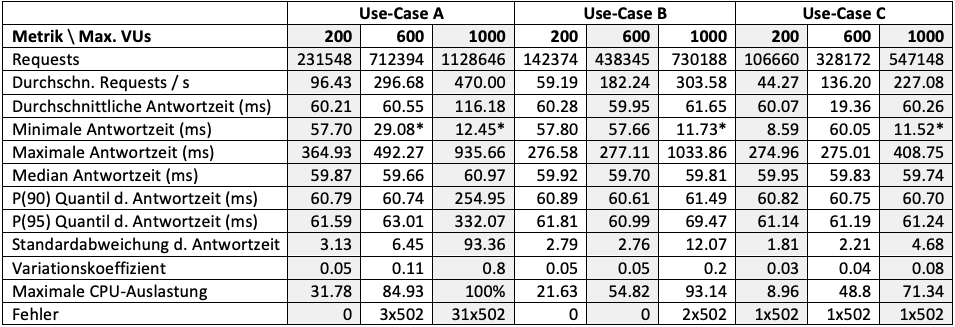
\includegraphics[width=\textwidth]{img/fargate128-stress-comparison.png}
    \caption[Fargate 128MB Stress-Test Vergleich]{Fargate 128MB Stress-Test Vergleich}
    \label{fig:fargate128-stress-comparison}
\end{figure}

Der erste Test wurde mit bis zu 200 Benutzern durchgeführt. Dabei konnte jedoch nur bis zu 32\% der CPU-Auslastung des Container-Clusters erreicht werden; In Use-Case B waren es sogar nur fast 22\%. Der geringen Auslastung entsprechend, war kaum eine Veränderung der Antwortzeiten gegenüber den Pipe-Clean Tests festzustellen (vgl. mit Abbildung \ref{fig:pipe128-comparison}). Einige Metriken lagen sogar unter den Grundwerten. Lediglich die maximale Antwortzeit hat sich bei allen Use-Cases, bspw. bei Use-Case A von 60,46ms auf 364,93ms, deutlich erhöht. Dies ist allerdings nur vereinzelt der Fall, da immer noch 95\% aller Anfragen innerhalb von ca. 62ms beantwortet werden und auch an der Standardabweichung hat sich nicht großartig verändert. 

Bei dem zweiten Stress-Test mit bis zu 600 VUs, änderte sich nicht viel im Vergleich zu dem Test mit 200 Benutzern. Es konnten zwar bis zu 84,93 Prozent CPU-Auslastung erreicht werden und die maximale Antwortzeit stieg erneut an, auf fast 500ms. Trotz dessen konnten von dem einzelnen Container 95\% der Anfragen innerhalb von knapp 63ms beantwortet werden. Problematisch zeigten sich hier drei Requests, die vom Server nicht mehr beantwortet werden konnten und den 502 Fehlercode zurücksendeten. Dies entspricht jedoch nur 0,00042\% aller in diesem Stress-Test durchgeführten Requests.

\begin{figure}[H]
    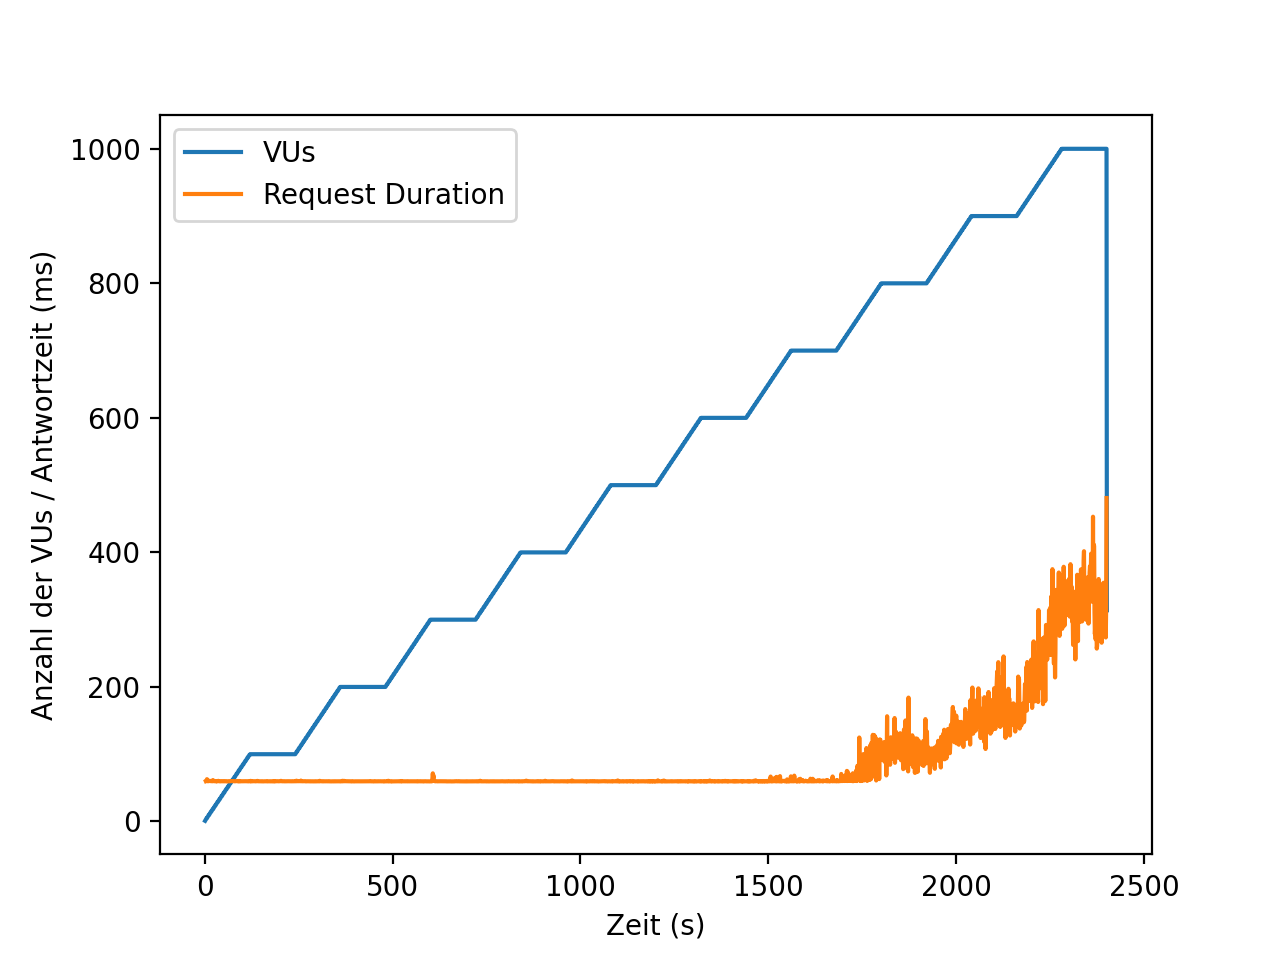
\includegraphics[width=\textwidth]{img/fargate128-stress1000.png}
    \caption[Container Stress-Test 1000VUs]{128MB Container Stress-Test 1000VUs Use-Case A}
    \label{fig:fargate128-stress1000}
\end{figure}

Der dritte Stress-Test für den 128MB Container wurde mit bis zu 1000 VUs durchgeführt. Abbildung \ref{fig:fargate128-stress1000} zeigt den zeitlichen Verlauf dieses Tests für Use-Case A. Es wird dabei die Anzahl der virtuellen Benutzer und die Antwortzeit im Median pro Sekunde dargestellt. Es wird deutlich, dass die Antwortzeit ab ca. 700 VUs deutlich ansteigt. Dies deckt sich der von AWS Cloudwatch gemessenen CPU-Auslastung von knapp unter 100\% die bei dieser Nutzerzahl gemessen wurde. In den Perioden mit konstanten Nutzerzahlen können die Requests besser verarbeitet werden und die Kurve geht wieder leicht herunter. Während des Tests wurden trotz einer CPU-Auslastung von teilweise 100\% nur 31 HTTP 502 Fehlercodes vom Server ausgelöst, was einer Quote von 0,0027\% entspricht. Die Antwortzeit konnte im Median weiterhin bei etwa 60ms gehalten werden; die durchschnittliche Antwortzeit stieg mit 116,8ms auf fast das doppelte des Grundwertes an.  
Bei Use-Case B lag die erreichte Prozessor-Auslastung bei 93,14\%. So wurden keine deutlichen Abweichungen ausgelöst. Die Standardabweichung stieg leicht an, liegt aber immer noch deutlich unter dem Wert des Pipe-Clean Tests der 128MB Lambda Funktion.

\subsubsection{Lambda}
Nachdem die maximale Performance des 128MB Containers ermittelt wurde, werden im Anschluss die gleichen Stress-Tests für die Lambda-Anwendung mit 128MB durchgeführt. Abbildung \ref{fig:lambda128-stress-comparison} zeigt die Ergebnisse. Für Use-Case A lässt sich erkennen, dass die Standardabweichung bei 200 und 600 VUs noch um die 19 beträgt, während bei 1000 Usern auf fast 55 ansteigt. Dies könnte allerdings an den extrem langen maximalen Antwortzeiten von bis zu 29.037ms liegen, die durch die Fehler verursacht werden. Die großen Fehler-Latenzen stehen im Gegensatz zu der Container Anwendung, bei der die maximale Antwortzeit immer noch knapp unter einer Sekunde lag. Auffallend ist, dass Fehler mit HTTP Statuscode 500 etwa 10s Antwortzeit aufweisen, während Fehler mit HTTP Statuscode 504 die fast 30s lange Latenz erzeugen. Die bei der Container-Anwendung erzeugten HTTP 502 Fehlercodes, führen stattdessen zu  Antwortzeiten von 12ms - 260ms. 

\begin{figure}[H]
    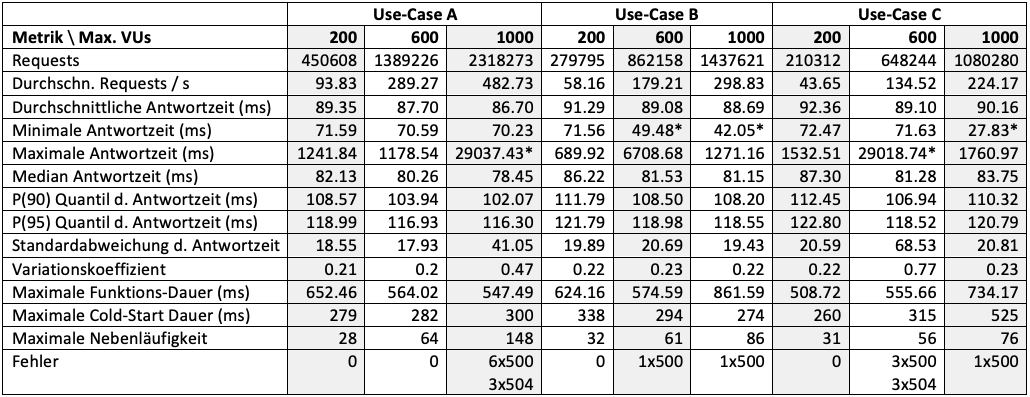
\includegraphics[width=\textwidth]{img/lambda128-stress-comparison.png}
    \caption[Lambda 128MB Stress-Test Vergleich]{Lambda 128MB Stress-Test Vergleich}
    \label{fig:lambda128-stress-comparison}
\end{figure}

Bei der Durchführung der Stress-Tests für die 128MB Lambda-Anwendung fällt außerdem auf, dass die Antwortzeit im Median bei steigenden Nutzerzahlen zu sinken scheint. Bei bis zu 200 VUs lag sie für Use-Case A noch bei 83.65ms, während sie bei bis zu 1000 VUs auf 77.89ms sank. Die Werte für Use-Case B scheinen einem ähnlichen Prinzip zu unterliegen. Es ist jedoch aktuell nicht bekannt, warum dies der Fall ist. Vermutlich provisioniert AWS die Funktionen schneller je mehr Anfragen sie erhalten. Trotz dessen, liegt die Antwortzeit im Median immer noch deutlich über der des 128MB Containers; die Differenz ist allerdings im Vergleich zu den Pipe-Clean Tests von 41,74ms auf 16.92ms gesunken (Use-Case A).

Zwischen den Use-Cases wird ebenfalls ein Unterschied in der Anzahl der nebenläufigen (concurrent) Lambda-Funktionen deutlich. Während bei 200 und 600 VUs für Use-Case B noch mehr Funktionen bereitgestellt wurden als für Use-Case A, zeigt sich für 1000 VUs ein umgekehrtes Bild. In diesem Fall, übertrifft der erste Use-Case den zweiten um 7 nebenläufige Funktionen. Dies ist interessant gegenüber RQ5, da es der Hypothese widerspricht, dass bei einer einzelnen angefragten Funktion weniger Coldstarts durchgeführt werden müssen als bei mehreren Funktionen (H5). Grund dafür ist vermutlich jedoch die geringere Anzahl der Requests pro Sekunde bei Use-Case B. 

\subsection{Spike-Test}
Für RQ2 soll die Performance unter schnell ansteigenden Nutzerzahlen ermittelt werde. Dazu wird ein Spike-Test durchgeführt. Ziel dessen ist es, die Performance der Anwendungen unter rasch ansteigender Last zu ermitteln. In den bisherigen Stress-Tests wurden nur langsame Anstiege (Ramp-Ups) durchgeführt. Nun soll nach einer kurzen Initialisierungsphase mit normalem Load (200VUs) eine schneller Anstieg auf 600 Virtuelle Benutzer erfolgen. Diese Benutzeranzahl wurde gewählt, um den Container nicht zu überlasten.

\subsubsection{Container}


\subsubsection{Lambda}
\chapter{Diskussion der Ergebnisse}
In diesem Kapitel sollen die Ergebnisse aus der vorangegangenen Analyse diskutiert werden.
\chapter{Fazit}
Im Rahmen dieser Bachelor-Thesis wurden Serverless-Funktionen mit AWS Lambda und Container-Anwendungen am Beispiel von AWS ECS mit Fargate auf ihre Performance untersucht und Kosten und Skalierungsverhalten analysiert. 

%*************************************************************************
% Backmatter
%*************************************************************************

% uncomment all following lines except the second for Appendix part
% do not forget to uncomment the Part 1 as well

\appendix
%\renewcommand{\thechapter}{\alph{chapter}}
\cleardoublepage
\part{Appendix}

% include all appendix chapters after this comment
\chapter{Appendix}


\section{Task-Definitionen}
Folgende Fargate Task-Definitionen wurden für die Container-Tests verwendet. In der Sektion "`containerDefinitions"' sind alle definierten Container, deren Container-Image, Arbeitsspeicher ("`memory"') und die Anzahl der vCPUs ("`cpu"') definiert. Außerhalb dieser Sektion sind die allgemeinen Werte dieses Tasks aufgeführt.

\subsection{128MB Container}
\begin{minted}[tabsize=2]{js}
{
  "ipcMode": null,
  "executionRoleArn": "arn:aws:iam::734730000614:role/ecsTaskExecutionRole",
  "containerDefinitions": [
    {
      "dnsSearchDomains": null,
      "environmentFiles": null,
      "logConfiguration": {
        "logDriver": "awslogs",
        "secretOptions": null,
        "options": {
          "awslogs-group": "/ecs/notes-express-task-definition",
          "awslogs-region": "eu-central-1",
          "awslogs-stream-prefix": "ecs"
        }
      },
      "entryPoint": [],
      "portMappings": [
        {
          "hostPort": 80,
          "protocol": "tcp",
          "containerPort": 80
        }
      ],
      "command": [],
      "linuxParameters": null,
      "cpu": 128,
      "environment": [],
      "resourceRequirements": null,
      "ulimits": null,
      "dnsServers": null,
      "mountPoints": [],
      "workingDirectory": null,
      "secrets": null,
      "dockerSecurityOptions": null,
      "memory": 128,
      "memoryReservation": null,
      "volumesFrom": [],
      "stopTimeout": null,
      "image": "734730000614.dkr.ecr.eu-central-1.amazonaws.com/notes-express:latest",
      "startTimeout": null,
      "firelensConfiguration": null,
      "dependsOn": null,
      "disableNetworking": null,
      "interactive": null,
      "healthCheck": null,
      "essential": true,
      "links": [],
      "hostname": null,
      "extraHosts": null,
      "pseudoTerminal": null,
      "user": null,
      "readonlyRootFilesystem": null,
      "dockerLabels": null,
      "systemControls": null,
      "privileged": null,
      "name": "custom"
    }
  ],
  "placementConstraints": [],
  "memory": "512",
  "taskRoleArn": null,
  "compatibilities": [
    "EC2",
    "FARGATE"
  ],
  "taskDefinitionArn": "arn:aws:ecs:eu-central-1:734730000614:task-definition/notes-express-task-definition:2",
  "family": "notes-express-task-definition",
  "requiresAttributes": [
    {
      "targetId": null,
      "targetType": null,
      "value": null,
      "name": "com.amazonaws.ecs.capability.logging-driver.awslogs"
    },
    {
      "targetId": null,
      "targetType": null,
      "value": null,
      "name": "ecs.capability.execution-role-awslogs"
    },
    {
      "targetId": null,
      "targetType": null,
      "value": null,
      "name": "com.amazonaws.ecs.capability.ecr-auth"
    },
    {
      "targetId": null,
      "targetType": null,
      "value": null,
      "name": "com.amazonaws.ecs.capability.docker-remote-api.1.19"
    },
    {
      "targetId": null,
      "targetType": null,
      "value": null,
      "name": "ecs.capability.execution-role-ecr-pull"
    },
    {
      "targetId": null,
      "targetType": null,
      "value": null,
      "name": "com.amazonaws.ecs.capability.docker-remote-api.1.18"
    },
    {
      "targetId": null,
      "targetType": null,
      "value": null,
      "name": "ecs.capability.task-eni"
    }
  ],
  "pidMode": null,
  "requiresCompatibilities": [
    "FARGATE"
  ],
  "networkMode": "awsvpc",
  "cpu": "256",
  "revision": 2,
  "status": "ACTIVE",
  "inferenceAccelerators": null,
  "proxyConfiguration": null,
  "volumes": []
}
\end{minted}

\section{256MB Container}
\begin{minted}[tabsize=2]{js}
{
  "ipcMode": null,
  "executionRoleArn": "arn:aws:iam::734730000614:role/ecsTaskExecutionRole",
  "containerDefinitions": [
    {
      "dnsSearchDomains": null,
      "environmentFiles": null,
      "logConfiguration": {
        "logDriver": "awslogs",
        "secretOptions": null,
        "options": {
          "awslogs-group": "/ecs/notes-express-task-definition",
          "awslogs-region": "eu-central-1",
          "awslogs-stream-prefix": "ecs"
        }
      },
      "entryPoint": [],
      "portMappings": [
        {
          "hostPort": 80,
          "protocol": "tcp",
          "containerPort": 80
        }
      ],
      "command": [],
      "linuxParameters": null,
      "cpu": 256,
      "environment": [],
      "resourceRequirements": null,
      "ulimits": null,
      "dnsServers": null,
      "mountPoints": [],
      "workingDirectory": null,
      "secrets": null,
      "dockerSecurityOptions": null,
      "memory": 256,
      "memoryReservation": null,
      "volumesFrom": [],
      "stopTimeout": null,
      "image": "734730000614.dkr.ecr.eu-central-1.amazonaws.com/notes-express:latest",
      "startTimeout": null,
      "firelensConfiguration": null,
      "dependsOn": null,
      "disableNetworking": null,
      "interactive": null,
      "healthCheck": null,
      "essential": true,
      "links": [],
      "hostname": null,
      "extraHosts": null,
      "pseudoTerminal": null,
      "user": null,
      "readonlyRootFilesystem": null,
      "dockerLabels": null,
      "systemControls": null,
      "privileged": null,
      "name": "custom"
    }
  ],
  "placementConstraints": [],
  "memory": "512",
  "taskRoleArn": null,
  "compatibilities": [
    "EC2",
    "FARGATE"
  ],
  "taskDefinitionArn": "arn:aws:ecs:eu-central-1:734730000614:task-definition/notes-express-task-definition-256:1",
  "family": "notes-express-task-definition-256",
  "requiresAttributes": [
    {
      "targetId": null,
      "targetType": null,
      "value": null,
      "name": "com.amazonaws.ecs.capability.logging-driver.awslogs"
    },
    {
      "targetId": null,
      "targetType": null,
      "value": null,
      "name": "ecs.capability.execution-role-awslogs"
    },
    {
      "targetId": null,
      "targetType": null,
      "value": null,
      "name": "com.amazonaws.ecs.capability.ecr-auth"
    },
    {
      "targetId": null,
      "targetType": null,
      "value": null,
      "name": "com.amazonaws.ecs.capability.docker-remote-api.1.19"
    },
    {
      "targetId": null,
      "targetType": null,
      "value": null,
      "name": "ecs.capability.execution-role-ecr-pull"
    },
    {
      "targetId": null,
      "targetType": null,
      "value": null,
      "name": "com.amazonaws.ecs.capability.docker-remote-api.1.18"
    },
    {
      "targetId": null,
      "targetType": null,
      "value": null,
      "name": "ecs.capability.task-eni"
    }
  ],
  "pidMode": null,
  "requiresCompatibilities": [
    "FARGATE"
  ],
  "networkMode": "awsvpc",
  "cpu": "256",
  "revision": 1,
  "status": "ACTIVE",
  "inferenceAccelerators": null,
  "proxyConfiguration": null,
  "volumes": []
}
\end{minted}

\section{512MB Container}
\begin{minted}[tabsize=2]{js}
{
  "ipcMode": null,
  "executionRoleArn": "arn:aws:iam::734730000614:role/ecsTaskExecutionRole",
  "containerDefinitions": [
    {
      "dnsSearchDomains": null,
      "environmentFiles": null,
      "logConfiguration": {
        "logDriver": "awslogs",
        "secretOptions": null,
        "options": {
          "awslogs-group": "/ecs/notes-express-task-definition",
          "awslogs-region": "eu-central-1",
          "awslogs-stream-prefix": "ecs"
        }
      },
      "entryPoint": [],
      "portMappings": [
        {
          "hostPort": 80,
          "protocol": "tcp",
          "containerPort": 80
        }
      ],
      "command": [],
      "linuxParameters": null,
      "cpu": 512,
      "environment": [],
      "resourceRequirements": null,
      "ulimits": null,
      "dnsServers": null,
      "mountPoints": [],
      "workingDirectory": null,
      "secrets": null,
      "dockerSecurityOptions": null,
      "memory": 512,
      "memoryReservation": null,
      "volumesFrom": [],
      "stopTimeout": null,
      "image": "734730000614.dkr.ecr.eu-central-1.amazonaws.com/notes-express:latest",
      "startTimeout": null,
      "firelensConfiguration": null,
      "dependsOn": null,
      "disableNetworking": null,
      "interactive": null,
      "healthCheck": null,
      "essential": true,
      "links": [],
      "hostname": null,
      "extraHosts": null,
      "pseudoTerminal": null,
      "user": null,
      "readonlyRootFilesystem": null,
      "dockerLabels": null,
      "systemControls": null,
      "privileged": null,
      "name": "custom"
    }
  ],
  "placementConstraints": [],
  "memory": "1024",
  "taskRoleArn": null,
  "compatibilities": [
    "EC2",
    "FARGATE"
  ],
  "taskDefinitionArn": "arn:aws:ecs:eu-central-1:734730000614:task-definition/notes-express-task-definition-512:1",
  "family": "notes-express-task-definition-512",
  "requiresAttributes": [
    {
      "targetId": null,
      "targetType": null,
      "value": null,
      "name": "com.amazonaws.ecs.capability.logging-driver.awslogs"
    },
    {
      "targetId": null,
      "targetType": null,
      "value": null,
      "name": "ecs.capability.execution-role-awslogs"
    },
    {
      "targetId": null,
      "targetType": null,
      "value": null,
      "name": "com.amazonaws.ecs.capability.ecr-auth"
    },
    {
      "targetId": null,
      "targetType": null,
      "value": null,
      "name": "com.amazonaws.ecs.capability.docker-remote-api.1.19"
    },
    {
      "targetId": null,
      "targetType": null,
      "value": null,
      "name": "ecs.capability.execution-role-ecr-pull"
    },
    {
      "targetId": null,
      "targetType": null,
      "value": null,
      "name": "com.amazonaws.ecs.capability.docker-remote-api.1.18"
    },
    {
      "targetId": null,
      "targetType": null,
      "value": null,
      "name": "ecs.capability.task-eni"
    }
  ],
  "pidMode": null,
  "requiresCompatibilities": [
    "FARGATE"
  ],
  "networkMode": "awsvpc",
  "cpu": "512",
  "revision": 1,
  "status": "ACTIVE",
  "inferenceAccelerators": null,
  "proxyConfiguration": null,
  "volumes": []
}
\end{minted}
\chapter{Repository}
\label{apx:repo}
In diesem Kapitel wird das Code-Repository erklärt.

%%************************************************
\chapter{Introduction to the ClassicThesis style}\label{ch:classicthesis}
%************************************************
The ClassicThesis bundle for \LaTeX\ has two goals:
\begin{enumerate}
    \item Provide students with an easy-to-use template for their
    Master's
    or PhD thesis. (Though it might also be used by other types of
    authors
    for reports, books, etc.)
    \item Provide a classic, high-quality typographic style that is
    inspired by \citeauthor{bringhurst:2002}'s ``\emph{The Elements of
    Typographic Style}'' \citep{bringhurst:2002}.
    \marginpar{\myTitle \myVersion}
\end{enumerate}
The bundle is configured to run with a \emph{full}
MiK\TeX\ or \TeX Live\footnote{See the file \texttt{LISTOFFILES} for
needed packages. Furthermore, \texttt{classicthesis}
works with most other distributions and, thus, with most systems
\LaTeX\ is available for.}
installation right away and, therefore, it uses only freely available
fonts. (Minion fans can easily adjust the style to their needs.)

People interested only in the nice style and not the whole bundle can
now use the style stand-alone via the file \texttt{classicthesis.sty}.
This works now also with ``plain'' \LaTeX.

As of version 3.0, \texttt{classicthesis} can also be easily used with
\mLyX\footnote{\url{http://www.lyx.org}} thanks to Nicholas Mariette
and Ivo Pletikosić. The \mLyX\ version of this manual will contain
more information on the details.

This should enable anyone with a basic knowledge of \LaTeXe\ or \mLyX\ to
produce beautiful documents without too much effort. In the end, this
is my overall goal: more beautiful documents, especially theses, as I
am tired of seeing so many ugly ones.

The whole template and the used style is released under the
\acsfont{GNU} General Public License.

If you like the style then I would appreciate a postcard:
\begin{center}
    André Miede \\
    Detmolder Straße 32 \\
    31737 Rinteln \\
    Germany
\end{center}
The postcards I received so far are available at:
\begin{center}
    \url{http://postcards.miede.de}
\end{center}
\marginpar{A well-balanced line width improves the legibility of
the text. That's what typography is all about, right?}
So far, many theses, some books, and several other publications have
been typeset successfully with it. If you are interested in some
typographic details behind it, enjoy Robert Bringhurst's wonderful book.
% \citep{bringhurst:2002}.

\paragraph{Important Note:} Some things of this style might look
unusual at first glance, many people feel so in the beginning.
However, all things are intentionally designed to be as they are,
especially these:
\begin{itemize}
    \item No bold fonts are used. Italics or spaced small caps do the
    job quite well.
    \item The size of the text body is intentionally shaped like it
    is. It supports both legibility and allows a reasonable amount of
    information to be on a page. And, no: the lines are not too short.
    \item The tables intentionally do not use vertical or double
    rules. See the documentation for the \texttt{booktabs} package for
    a nice discussion of this topic.\footnote{To be found online at
    \url{http://mirror.ctan.org/macros/latex/contrib/booktabs/}.}
    \item And last but not least, to provide the reader with a way
    easier access to page numbers in the table of contents, the page
    numbers are right behind the titles. Yes, they are \emph{not}
    neatly aligned at the right side and they are \emph{not} connected
    with dots that help the eye to bridge a distance that is not
    necessary. If you are still not convinced: is your reader
    interested in the page number or does she want to sum the numbers
    up?
\end{itemize}
Therefore, please do not break the beauty of the style by changing
these things unless you really know what you are doing! Please.

\paragraph{Yet Another Important Note:} Since \texttt{classicthesis}'
first release in 2006, many things have changed in the \LaTeX\ world.
Trying to keep up-to-date, \texttt{classicthesis} grew and evolved
into many directions, trying to stay (some kind of) stable and be
compatible with its port to \mLyX. However, there are still many
remains from older times in the code, many dirty workarounds here and
there, and several other things I am absolutely not proud of (for
example my unwise combination of \acsfont{KOMA} and
\texttt{titlesec} etc.).
\graffito{An outlook into the future of \texttt{classicthesis}.}

Currently, I am looking into how to completely re-design and
re-implement \texttt{classicthesis} making it easier to maintain and
to use. As a general idea, \texttt{classicthesis.sty} should be
developed and distributed separately from the template bundle itself.
Excellent spin-offs such as \texttt{arsclassica} could also be
integrated (with permission by their authors) as format configurations.
Also, current trends of \texttt{microtype}, \texttt{fontspec}, etc.
should be included as well. As I am not really into deep
\LaTeX\ programming,
I will reach out to the \LaTeX\ community for their expertise and help.


\section{Organization}
A very important factor for successful thesis writing is the
organization of the material. This template suggests a structure as
the following:
\begin{itemize}
    \marginpar{You can use these margins for summaries of the text
    body\dots}
    \item\texttt{Chapters/} is where all the ``real'' content goes in
    separate files such as \texttt{Chapter01.tex} etc.
    % \item\texttt{Examples/} is where you store all listings and other
    % examples you want to use for your text.
    \item\texttt{FrontBackMatter/} is where all the stuff goes that
    surrounds the ``real'' content, such as the acknowledgments,
    dedication, etc.
    \item\texttt{gfx/} is where you put all the graphics you use in
    the thesis. Maybe they should be organized into subfolders
    depending on the chapter they are used in, if you have a lot of
    graphics.
    \item\texttt{Bibliography.bib}: the Bib\TeX\ database to organize
    all the references you might want to cite.
    \item\texttt{classicthesis.sty}: the style definition to get this
    awesome look and feel. Does not only work with this thesis template
    but also on its own (see folder \texttt{Examples}). Bonus: works
    with both \LaTeX\ and \textsc{pdf}\LaTeX\dots and \mLyX.
    % \item\texttt{ClassicThesis.tcp} a \TeX nicCenter project file.
    Great tool and it's free!
    \item\texttt{ClassicThesis.tex}: the main file of your thesis
    where all gets bundled together.
    \item\texttt{classicthesis-config.tex}: a central place to load all
    nifty packages that are used. % In there, you can also activate
    % backrefs in order to have information in the bibliography about
    % where a source was cited in the text (\ie, the page number).

    \emph{Make your changes and adjustments here.} This means that you
    specify here the options you want to load \texttt{classicthesis.sty}
    with. You also adjust the title of your thesis, your name, and all
    similar information here. Refer to \autoref{sec:custom} for more
    information.

    This had to change as of version 3.0 in order to enable an easy
    transition from the ``basic'' style to \mLyX.
\end{itemize}
In total, this should get you started in no time.


\clearpage
\section{Style Options}\label{sec:options}
There are a couple of options for \texttt{classicthesis.sty} that
allow for a bit of freedom concerning the layout:
\marginpar{\dots or your supervisor might use the margins for some
    comments of her own while reading.}
\begin{itemize}
    \item General:
        \begin{itemize}
            \item\texttt{drafting}: prints the date and time at the bottom of
            each page, so you always know which version you are dealing with.
            Might come in handy not to give your Prof. that old draft.
        \end{itemize}

    \item Parts and Chapters:
        \begin{itemize}
            \item\texttt{parts}: if you use Part divisions for your document,
            you should choose this option. (Cannot be used together with
            \texttt{nochapters}.)

            \item\texttt{linedheaders}: changes the look of the chapter
            headings a bit by adding a horizontal line above the chapter
            title. The chapter number will also be moved to the top of the
            page, above the chapter title.
        \end{itemize}

    \item Typography:
        \begin{itemize}
            \item\texttt{eulerchapternumbers}: use figures from Hermann Zapf's
            Euler math font for the chapter numbers. By default, old style
            figures from the Palatino font are used.

            \item\texttt{beramono}: loads Bera Mono as typewriter font.
            (Default setting is using the standard CM typewriter font.)

            \item\texttt{eulermath}: loads the awesome Euler fonts for math.
            Pala\-tino is used as default font.
        \end{itemize}

    \marginpar{Options are enabled via \texttt{option=true}}

    \item Table of Contents:
        \begin{itemize}
            \item\texttt{tocaligned}: aligns the whole table of contents on
            the left side. Some people like that, some don't.

            \item\texttt{dottedtoc}: sets pagenumbers flushed right in the
            table of contents.

            \item\texttt{manychapters}: if you need more than nine chapters for
            your document, you might not be happy with the spacing between the
            chapter number and the chapter title in the Table of Contents.
            This option allows for additional space in this context.
            However, it does not look as ``perfect'' if you use
            \verb|\parts| for structuring your document.
        \end{itemize}

    \item Floats:
        \begin{itemize}
            \item\texttt{listings}: loads the \texttt{listings} package (if not
            already done) and configures the List of Listings accordingly.

            \item\texttt{floatperchapter}: activates numbering per chapter for
            all floats such as figures, tables, and listings (if used).
        \end{itemize}

\end{itemize}

Furthermore, pre-defined margins for different paper sizes are available, \eg, \texttt{a4paper}, \texttt{a5paper}, and \texttt{letterpaper}. These are based on your chosen option of \verb|\documentclass|.

The best way to figure these options out is to try the different
possibilities and see what you and your supervisor like best.

In order to make things easier, \texttt{classicthesis-config.tex}
contains some useful commands that might help you.


\section{Customization}\label{sec:custom}
%(As of v3.0, the Classic Thesis Style for \LaTeX{} and \mLyX{} share
%the same two \texttt{.sty} files.)
This section will show you some hints how to adapt
\texttt{classicthesis} to your needs.

The file \texttt{classicthesis.sty}
contains the core functionality of the style and in most cases will
be left intact, whereas the file \texttt{classic\-thesis-config.tex}
is used for some common user customizations.

The first customization you are about to make is to alter the document
title, author name, and other thesis details. In order to do this, replace
the data in the following lines of \texttt{classicthesis-config.tex:}%
\marginpar{Modifications in \texttt{classic\-thesis-config.tex}%
}

\begin{lstlisting}
    % **************************************************
    % 2. Personal data and user ad-hoc commands
    % **************************************************
    \newcommand{\myTitle}{A Classic Thesis Style\xspace}
    \newcommand{\mySubtitle}{An Homage to...\xspace}
\end{lstlisting}

Further customization can be made in \texttt{classicthesis-config.tex}
by choosing the options to \texttt{classicthesis.sty}
(see~\autoref{sec:options}) in a line that looks like this:

\begin{lstlisting}
  \PassOptionsToPackage{
    drafting=true,    % print version information on the bottom of the pages
    tocaligned=false, % the left column of the toc will be aligned (no indentation)
    dottedtoc=false,  % page numbers in ToC flushed right
    parts=true,       % use part division
    eulerchapternumbers=true, % use AMS Euler for chapter font (otherwise Palatino)
    linedheaders=false,       % chaper headers will have line above and beneath
    floatperchapter=true,     % numbering per chapter for all floats (i.e., Figure 1.1)
    listings=true,    % load listings package and setup LoL
    subfig=true,      % setup for preloaded subfig package
    eulermath=false,  % use awesome Euler fonts for mathematical formulae (only with pdfLaTeX)
    beramono=true,    % toggle a nice monospaced font (w/ bold)
    minionpro=false   % setup for minion pro font; use minion pro small caps as well (only with pdfLaTeX)
  }{classicthesis}
\end{lstlisting}

Many other customizations in \texttt{classicthesis-config.tex} are
possible, but you should be careful making changes there, since some
changes could cause errors.

% Finally, changes can be made in the file \texttt{classicthesis.sty},%
% \marginpar{Modifications in \texttt{classicthesis.sty}%
% } although this is mostly not designed for user customization. The
% main change that might be made here is the text-block size, for example,
% to get longer lines of text.


\section{Issues}\label{sec:issues}
This section will list some information about problems using
\texttt{classic\-thesis} in general or using it with other packages.

Beta versions of \texttt{classicthesis} can be found at Bitbucket:
\begin{center}
    \url{https://bitbucket.org/amiede/classicthesis/}
\end{center}
There, you can also post serious bugs and problems you encounter.


\section{Future Work}
So far, this is a quite stable version that served a couple of people
well during their thesis time. However, some things are still not as
they should be. Proper documentation in the standard format is still
missing. In the long run, the style should probably be published
separately, with the template bundle being only an application of the
style. Alas, there is no time for that at the moment\dots it could be
a nice task for a small group of \LaTeX nicians.

Please do not send me email with questions concerning \LaTeX\ or the
template, as I do not have time for an answer. But if you have
comments, suggestions, or improvements for the style or the template
in general, do not hesitate to write them on that postcard of yours.


\section{Beyond a Thesis}
The layout of \texttt{classicthesis.sty} can be easily used without the
framework of this template. A few examples where it was used to typeset
an article, a book or a curriculum vitae can be found in the folder
\texttt{Examples}. The examples have been tested with
\texttt{latex} and \texttt{pdflatex} and are easy to compile. To
encourage you even more, PDFs built from the sources can be found in the
same folder.


\section{License}
\paragraph{GNU General Public License:} This program is free software;
you can redistribute it and/or modify
it under the terms of the \acsfont{GNU} General Public License as
published by
the Free Software Foundation; either version 2 of the License, or
(at your option) any later version.

This program is distributed in the hope that it will be useful,
but \emph{without any warranty}; without even the implied warranty of
\emph{merchant\-ability} or \emph{fitness for a particular purpose}.
See the
\acsfont{GNU} General Public License for more details.

You should have received a copy of the \acsfont{GNU} General
Public License
along with this program; see the file \texttt{COPYING}.  If not,
write to
the Free Software Foundation, Inc., 59 Temple Place - Suite 330,
Boston, MA 02111-1307, USA.

\paragraph{classichthesis Authors' note:} There have been some discussions about the GPL's implications on using \texttt{classicthesis} for theses etc. Details can be found here:
\begin{center}
  \url{https://bitbucket.org/amiede/classicthesis/issues/123/}
\end{center}

We chose (and currently stick with) the GPL because we would not like to compete with proprietary modified versions of our own work. However, the whole template is free as free beer and free speech. We will not demand the sources for theses, books, CVs, etc. that were created using \texttt{classicthesis}.

Postcards are still highly appreciated.





%*****************************************
%*****************************************
%*****************************************
%*****************************************
%*****************************************

%%********************************************************************
% Appendix
%*******************************************************
% If problems with the headers: get headings in appendix etc. right
%\markboth{\spacedlowsmallcaps{Appendix}}{\spacedlowsmallcaps{Appendix}}
\chapter{Appendix Test}
Lorem ipsum at nusquam appellantur his, ut eos erant homero
concludaturque. Albucius appellantur deterruisset id eam, vivendum
partiendo dissentiet ei ius. Vis melius facilisis ea, sea id convenire
referrentur, takimata adolescens ex duo. Ei harum argumentum per. Eam
vidit exerci appetere ad, ut vel zzril intellegam interpretaris.
\graffito{More dummy text.}

%Errem omnium ea per, pro congue populo ornatus cu, ex qui dicant
%nemore melius. No pri diam iriure euismod. Graecis eleifend
%appellantur quo id. Id corpora inimicus nam, facer nonummy ne pro,
%kasd repudiandae ei mei. Mea menandri mediocrem dissentiet cu, ex
%nominati imperdiet nec, sea odio duis vocent ei. Tempor everti
%appareat cu ius, ridens audiam an qui, aliquid admodum conceptam ne
%qui. Vis ea melius nostrum, mel alienum euripidis eu.

\section{Appendix Section Test}
Test: \autoref{tab:moreexample} (This reference should have a
lowercase, small caps \spacedlowsmallcaps{A} if the option
\texttt{floatperchapter} is activated, just as in the table itself
 $\rightarrow$ however, this does not work at the moment.)

\begin{table}[h]
    \myfloatalign
    \begin{tabularx}{\textwidth}{Xll} \toprule
        \tableheadline{labitur bonorum pri no} & \tableheadline{que vista}
        & \tableheadline{human} \\ \midrule
        fastidii ea ius & germano &  demonstratea \\
        suscipit instructior & titulo & personas \\
        %postulant quo & westeuropee & sanctificatec \\
        \midrule
        quaestio philosophia & facto & demonstrated \\
        %autem vulputate ex & parola & romanic \\
        %usu mucius iisque & studio & sanctificatef \\
        \bottomrule
    \end{tabularx}
    \caption[Autem usu id]{Autem usu id.}
    \label{tab:moreexample}
\end{table}

%Nulla fastidii ea ius, exerci suscipit instructior te nam, in ullum
%postulant quo. Congue quaestio philosophia his at, sea odio autem
%vulputate ex. Cu usu mucius iisque voluptua. Sit maiorum propriae at,
%ea cum primis intellegat. Hinc cotidieque reprehendunt eu nec. Autem
%timeam deleniti usu id, in nec nibh altera.




\section{Another Appendix Section Test}
Equidem detraxit cu nam, vix eu delenit periculis. Eos ut vero
constituto, no vidit propriae complectitur sea. Diceret nonummy in
has, no qui eligendi recteque consetetur. Mel eu dictas suscipiantur,
et sed placerat oporteat. At ipsum electram mei, ad aeque atomorum
mea. There is also a useless Pascal listing below: \autoref{lst:useless}.

\begin{lstlisting}[float=b,language=Pascal,frame=tb,caption={A floating example (\texttt{listings} manual)},label=lst:useless]
for i:=maxint downto 0 do
begin
{ do nothing }
end;
\end{lstlisting}

%Ei solet nemore consectetuer nam. Ad eam porro impetus, te choro omnes
%evertitur mel. Molestie conclusionemque vel at, no qui omittam
%expetenda efficiendi. Eu quo nobis offendit, verterem scriptorem ne
%vix.



%*************************************************************************
% Other Stuff in the Back
%*************************************************************************
\cleardoublepage%********************************************************************
% Bibliography
%*******************************************************
% work-around to have small caps also here in the headline
% https://tex.stackexchange.com/questions/188126/wrong-header-in-bibliography-classicthesis
% Thanks to Enrico Gregorio
\defbibheading{bibintoc}[\bibname]{%
  \phantomsection
  \manualmark
  \markboth{\spacedlowsmallcaps{#1}}{\spacedlowsmallcaps{#1}}%
  \addtocontents{toc}{\protect\vspace{\beforebibskip}}%
  \addcontentsline{toc}{chapter}{\tocEntry{#1}}%
  \chapter*{#1}%
}
\printbibliography[heading=bibintoc]

%*************************************************************************
% Game Over: Restore, Restart, or Quit?
%*************************************************************************
\end{document}
%*************************************************************************
